%
%
\documentclass{article}
\usepackage{amsmath}
\usepackage{amsthm}
\usepackage{empheq}
\usepackage{graphicx}
\usepackage{bm}
\usepackage{framed}
\usepackage{enumerate}
\usepackage{array}
\usepackage{tikz}
\usepackage{caption}
\usepackage{amsfonts}
\usepackage[margin=3cm]{geometry}
\usepackage{float}

\usetikzlibrary{arrows}

\newcommand{\cO}{\mathcal{O}}                               %
\newcommand{\domain}{\mathcal{D}}                           %
\newcommand{\example}{\textbf{Example:}}                    %
\newcommand{\examples}{\textbf{Examples:}}                  %
\newcommand{\definition}{\textbf{Definition:}}              %
\newcommand{\theorem}{\textbf{Theorem:}}                    %
\newcommand{\corollary}{\textbf{Corollary:}}                %
\newcommand{\lemma}{\textbf{Lemma:}}                        %
\newcommand{\bp}{\bm{\phi}}                                 % These are used a lot!
\newcommand{\bx}{\bm{x}}                                    %
\newcommand{\rtwo}{\mathbb{R}^2}                            %
\newcommand{\xeq}[1] { \dot{\bm{ #1 }} = \bm{f}(\bm{ #1}) } %
\newcommand{\pder}[2] {\frac{\partial {#1}}{\partial {#2} }}%

\begin{document}

\title{Dynamical Systems}
\author{Course given by Prof. J.Lister \\
\LaTeX\  by Dominic Skinner \\
Dom-Skinner@github.com}
\maketitle
\tableofcontents
\section*{Introduction}
A dynamical system is a set of equations describing the evolution of a system
with respect to a time-like variable. Usually they are non-linear.
\\
The possible states of the system define the state space/phase space.
\\
\\
\example\   The logistic map
\[ x_{n+1} = \mu x_n ( 1- x_n) \]
For $ 0 \leq \mu \leq 4 $ this describes evolution with respect to a discrete time 
$n$ in a state space $[0,1]$.
\\
\\
\example\   The Lotka-Voltera equations
\begin{align*}
\dot{r} &= r(a - br -cs) \\
\dot{s} &= s(d - er -fs)
\end{align*}
Where \emph{a-f} are positive constants. These describe continous evolution 
in a state space $(r,s) \in [0 , \infty] \times [0, \infty]$ as a model for 
the population of two species competing for the same food supply.
\\
\\
\example\   The non-linear Schr\"odinger equation
\[ i \frac{\partial \Psi}{ \partial t} = \nabla^2 \Psi + |\Psi|^2 \Psi \]
This describes evolution in an infinite dimensional statespace of possible
wavefunctions.
\\
\\
Because the equations are non-linear, it is often impossible to find a complete
set of closed form analytic solutions. Instead, we resort to a mixture of 
geometric and analytic arguments, and aim to say something about the generic
long-term behaviour.
\\
\\
\example\   
\begin{align*}
\dot{r} &= r(3 - r -s) \\
\dot{s} &= s(2 - r -s)
\end{align*}
Consider the regions where $\dot{r}$ and $\dot{s}$ are $>0, \; <0, \; =0$. 
\\
If $r,s >0$ then
\begin{align*}
r+s &< 2 \implies \dot{r}, \dot{s} > 0 \\
2 < r+s &< 3 \implies \dot{r} >0 , \; \dot{s} < 0 \\
r+s &> 3 \implies \dot{r}, \dot{s} < 0 \\
\end{align*}
$\dot{r} = 0$ if $r=0$ or $r+s = 3$. \\
$\dot{s} = 0$ if $s=0$ or $r+s = 2$. \\
Therefore $\dot{r} = \dot{s} = 0$ at the fixed points $(0,0), \; (3,0), \; (0,2)$.
This gives the phase portrait/diagram/plane%
\footnote{Phase portrait, phase diagram, phase plane will be used interchangably}
\begin{figure}[H]
\begin{minipage}[c]{0.35\linewidth}
\includegraphics{Fig1.pdf}
\end{minipage}
\begin{minipage}[c]{0.55\linewidth}
The most important feature of the phase portrait is that all solutions with 
$r >0$ tend to the stable fixed point $(3,0)$. The fixed points $(0,0)$ and
$(0,2)$ are unstable. There are no periodic orbits.
\end{minipage}
\end{figure}
\noindent
\example\   
\begin{align*}
\dot{r} &= r(3 - r -s) \\
\dot{s} &= s(2 - \mu r -s)
\end{align*}
In this case, a new fixed point 
$\displaystyle \left(\frac{1}{1- \mu} , \frac{2 - 3 \mu}{1- \mu} \right)$
appears in the state space at $\mu = \frac{2}{3}$ and for $\mu < \frac{2}{3}$ 
is the long term stable attractor. 
\\
A qualitative change in the solution structure is called a bifurcation.
\\
\\
\example\   
\begin{align*}
\dot{x} &= -y + \epsilon x (\mu - x^2 - y^2) \\
\dot{y} &= \;\;\; x + \epsilon y (\mu - x^2 - y^2)
\end{align*}
Use polar coordinates which are a more natural choice for this problem.
In general:
\begin{empheq}[box=\fbox]{align}
\dot{r} &= \frac{x \dot{x} + y \dot{y}}{r} \nonumber \\
\dot{\theta} &= \frac{x \dot{y} - y \dot{x} }{ r^2} \nonumber
\end{empheq}
Which are equations that will be referred to frequently. \footnote{so learn them now!}
In our example, they become
\begin{align*}
\dot{r} &= \epsilon r (\mu - r^2) \\
\dot{\theta} &= 1
\end{align*}
Consider $\dot{r}$ and $\dot{\theta}$:
\begin{center}
\includegraphics{Fig4.pdf}
\end{center}
\noindent
The infinite set of periodic solutions for $\epsilon = 0$ is destroyed by any 
perturbation to $\epsilon \neq 0$. This is an example of structural instability.
If $\mu > 0$ then just one limit cycle survives and is stable (unstable) for 
$\epsilon >0$ ($\epsilon < 0$). The appearance of the limit cycle as $\mu \uparrow$ 
through $0$ is another form of bifurcation.
\\
\\
\example\ In 2D the points of successive interection $x_n$ of a 
solution near a limit cycle with a line $\varepsilon$ perpendicular to the cycle,
move monotonically towards/away from the point of intersection $x^{*}$ of 
$\varepsilon$ with the limit cycle.
% INSERT PLOT HERE
\begin{figure}[H]
\centering
\includegraphics[width=7cm, height=4cm]{fig2.png}
\end{figure}
\noindent
The point $x^{*}$ is a stable/unstable fixed point of this Poincar\'e recurrence
map.
\\
In 3 or higher dimensions, or in 2D with time-dependent coefficients there is 
room for much more complicated behaviour including \underline{chaos}.
%%%%%%%%%%%%%CHAPTER 1
\section{Basic Definitions}
We need some termonology.
\subsection{Notation}
We only consider ODEs of the form 
\begin{equation}\tag{*}
\xeq{x}
\end{equation}
for \textbf{x} in a phase space/state space $E \subset \mathbb{R}^{n}$.
The n first order ODEs form a dynamical system of order (dimension) n.
\\
\\
Since
\[ \frac{\partial \textbf{f} } { \partial t} = 0 \]
 we call the system \underline{autonomous}.
\\
\\
A non-autonomous system $\dot{\textbf{x}} = \textbf{f}(\textbf{x} ,t) $ can be
made autonomous by setting
\[ \textbf{y} = ( \textbf{x},t) \quad \mbox{ with } \quad \dot{\textbf{y}} = ( \textbf{f}(\textbf{y}),1) \]
The n$^{th}$ order ODE
\[ \frac{d ^n x}{d t^n} = g \left( x , \frac{d x}{d t} , \dots , \frac{d^{n-1} x}{d t^{n-1}} \right) \]
can be put in the form (*) by setting
\[ \textbf{y} =  \left( x , \frac{d x}{d t} , \dots , \frac{d^{n-1} x}{d t^{n-1}} \right) \]
with 
\[ \dot{\textbf{y}} =  \left( y_2 , y_3 , \dots , g( \textbf{y}) \right) \]
Similarly we will consider maps in the form
\[ \textbf{x}_{n+1} = \textbf{F}(\textbf{x}_n) \]
\subsection{Initial Value Problem}
Consider the IVP: 
\[ \dot{\textbf{x}} = \textbf{f}(\textbf{x})  \]
\[ \textbf{x}(t_0)  = \textbf{x}_0\]
In Analysis II we showed that if $\textbf{f}$ satisfies a Lipshitz condition
then we are guaranteed that a solution exists in a neighbourhood of $\textbf{x}_0$,
$ t_0$ and is unique.
\\
(Lipshitz condition is that $\exists$ $L$, $a$, s.t. 
$|\textbf{f}(\textbf{x})- \textbf{f}(\textbf{x})| < L|\textbf{x} - \textbf{y}|$
$, \quad \forall \; |\textbf{x}-\textbf{x}_0|, \; |\textbf{y}-\textbf{x}_0| < a$.)
\\
\\
Moreover, solutions $\textbf{x}(t \, ; \textbf{x}')$ to 
\[ \dot{\textbf{x}} = \textbf{f}(\textbf{x})  \]
\[ \textbf{x}(t_0)  = \textbf{x}'\]
exist, are unique and they depend continously on $\textbf{x}' , \, t$.
\\
\\
Note we are not guaranteed existence for all times.
\\
\\
\example\ 
\[ \dot{x} = x^2  \]
\[ x(0)  = 1\]
This has solution
\[ x(t) = \frac{1}{1-t} \]
and so $x \to \infty$ as $t \uparrow 1$.
\\
\\
If $|\textbf{x}(t)| \to \infty$ as $t \to T \;(< \infty)$ then we call this
finite time blow up.
\\
\\
\example\ Non-uniqueness when $\textbf{f}$ is non-Lipshitz. If
\[ \dot{x} = \left\{\begin{array}{lr}
				\sqrt{x} & \mbox{for } x >0 \\
				0        & \mbox{for } x \leq 0
				\end{array}
\right. \mbox{ and } x(0) = 0 \]
Then there is a family of solutions
\[ \left. \begin{array}{lr} 
				x = 0 & t < \tau \\
				x = \frac{1}{4}(t - \tau)^2 & t > \tau
\end{array} \right\} \mbox{ for any } \tau \geq 0 \]
From now on we will assume that \textbf{f} is differentiable ( and so Lipshitz).
\\
\subsection{Trajectories and Flows}
Consider the autonomous system
$ \dot{\textbf{x}} = \textbf{f}(\textbf{x}) $
The solution $\textbf{x}(t)$ to the IVP with $\textbf{x}(0) = \textbf{x}_0$
defines a trajectory. (orbit/integral curve)
\\
\\
The distance travelled along this curve clearly only depends on $t - t_0$, 
and we could consider lots of starting points $\textbf{x}_0$.
\\
This motivates the idea of a flow. 
\\
\\
\definition\ (Flow) \\
Given \textbf{f}, the corresponding flow is defined to be a (the) function
$\bp_t (\textbf{x}) $ from $E \times \mathbb{R} \to E$ such that
\[ 
\frac{\partial}{\partial t} \bp_t ( \bm{x} ) = \bm{f}(\bp_t (\bm{x} ) ), \qquad\
\bp_0(\bm{x}) = \bm{x} 
 \]
The solution to the IVP $\dot{\bm{x}} = \bm{f}(\bm{x}), \; \bm{x}(t_0) = \bm{x}_0$,
is just $\bm{x}(t) = \bp_{t - t_0} (\bm{x}_0)$
\\
Clearly 
\[ \bp_{s+t}(\bm{x}) = \bp_s(\bp_t(\bm{x})) = \bp_t ( \bp_s (\bm{x} ) ) \]
\begin{framed}
\noindent Aside: We can establish another link with maps, by defining 
$\bm{x}_{n+1} = \bm{F}(\bm{x}_n) = \bp_{\Delta t} (\bm{x}_n)$. \\
Clearly $\bp_{n \Delta t} (\bm{x} ) = \bm{F} ( \bp_{(n-1) \Delta t} (\bm{x} )) = \bm{F}^n(\bm{x}) $ 
\end{framed}
\subsection{Flows, Trajectories, Orbits, Invariant Sets, \& Limiting Sets}
Using the idea of a flow, we define the following:
\\
\\
\definition\ Orbits/Trajectories
\\
 The orbit of $\bp_t(\bm{x})$ through $\bm{x}_0$ is
the set $\cO(\bm{x}_0) = \{ \bp_t(\bm{x}_0): -\infty < t < \infty \}$.
\\
The forwards (backwards) orbit is 
\[\cO^{+ \, (-)}(\bm{x}_0) = \{ \bp_t(\bm{x}_0):  t \geq 0 \; (t \leq 0) \} \]
\definition\ Invariant sets
\\
A set of points $\Lambda \subset E$ is invariant if
$\bm{x} \in \Lambda \implies \cO(\bm{x}) \subset \Lambda$
\\
Clearly $\cO(\bm{x}_0)$ is invariant, and so is any union of orbits.
\\
\\
Particular cases of interest are
\\
\\
\definition\ Fixed points
\\
$\bm{x}_0$ is a periodic point with period $T$ if $\bp_T(\bm{x}_0)= \bm{x}_0$
for some $T>0$ and $\bp_t (\bm{x}_0) \neq \bm{x}_0$ for $0 < t < T$.
The set $ \{ \bp_t ( \bm{x}_0) : 0 \leq t < T \}$ is the periodic orbit
through $\bm{x}_0$.
\\
\\
\definition\ Limit Cycle
\\
A limit cycle is an isolated periodic orbit, i.e. there are no other periodic
orbits within a sufficiently small neighbourhood.
\\
\\
\definition\ Homoclinic and Heteroclinic orbits
\\
If $\bm{x}_0$ is a fixed point and $\exists \; \bm{y} \neq \bm{x}_0$ such that
$\bp_t(\bm{y}) \to \bm{x}_0$ as $t \to \pm \infty$ then 
$\cO(\bm{y})$ is a homoclinic orbit.
\\
\\
If $\bm{x}_0$, $\bm{x}_1$ are fixed points and 
$\exists \; \bm{y} \neq \bm{x}_0 , \, \bm{x}_1$ with $\bp_t (\bm{y}) \to \bm{x}_0$
as $t \to - \infty$, $\bp_t(\bm{y}) \to \bm{x}_1$ as $t \to + \infty$ then
$\cO(\bm{y})$ is a heteroclinic orbit.
%
\begin{figure}[H]
\centering\caption*{Example of a Heteroclinic and a Homoclinic orbit}
\includegraphics[width=4cm, height=6cm]{fig3.png}
\end{figure}
\noindent If we are interested in the long-term behaviour of trajectories, it is not 
enough simply to think of 
\[ \lim_{t \to \infty} \bp_t(\bm{x}) \]
because the limit might not exist; for example a limit cycle.
\\
\\
\definition\ Limit set
\\
The $\omega$-limit set of $\bm{x}$ is 
\[ \omega (\bm{x}) = \{ \bm{y} : \exists \mbox{ a sequence } (t_n) \mbox{ with }\
 \bp_{t_n}(\bm{x}) \to \bm{y} \mbox{ and } t_n \to \infty \} \]
Similarly the $\alpha$ limit set is defined by sequences with $t_n \to - \infty$.
\\
\\
\example\ \\
\begin{minipage}[c][0.22\textwidth][c]{0.2\textwidth}
\end{minipage}
\hspace{0.2\textwidth}
\begin{minipage}[c][0.22\textwidth][c]{0.3\textwidth}
\begin{center}
\includegraphics{Fig5.pdf}
\end{center}
\end{minipage}
%
\begin{minipage}[c][0.22\textwidth][c]{0.3\textwidth}
\begin{center}
$ \begin{array}{rl}
\dot{r} &= r(1-r^2) \\
\dot{\theta} &= 1
\end{array}$
\end{center}
\end{minipage}
\\
%
For $\bm{x}$ with $0 < |\bm{x}| < 1$ we have that
\[ \omega ( \bm{x} ) = \{ \bm{y} : |\bm{y}| = 1 \}  \qquad  \alpha ( \bm{x} ) = \{\bm{0} \} \]
For $|\bm{x}|>1$
\[ \omega ( \bm{x} ) = \{ \bm{y} : |\bm{y}| = 1 \}  \qquad  \alpha ( \bm{x} ) = \{ \} \]
\\
\\
In fact, the limit sets are always invariant sets since
\begin{itemize}
\item If $\cO(\bm{x})$ is bounded then $\omega(\bm{x})$ is non-empty.
\item If $\bp_t(\bm{x}) \to \infty$ then $\omega(\bm{x}) = \{ \} $.
\end{itemize}\vspace{3mm}
\definition\ (For maps) 
\\
Fixed points solve $\bm{F}(\bm{x}) = \bm{x}$. Orbits, periodic points etc.
are defined as above by replacing $\bp_t(\bm{x})$ by $\bm{F}^n(\bm{x})$,
etc.
\\
\\
A periodic orbit with period N is called an N-cycle.
\subsection{Topological equivalence and structural stability of flows}
This section is in a handout.
\\
\section{Flow near fixed points}
The simplest features of a flow are the fixed points. Find them by first 
solving $\bm{F}(\bm{x}) = \bm{0}$.
\\
\subsection{Linearisation}
If $\bm{f}$ is sufficiently smooth and $\bm{x}_0$ is a fixed point, we expand
in a Taylor series with $\bm{f}(\bm{x}_0)=\bm{0}$ to obtain 
\[\dot{\bm{y}} = A\bm{y} + O(|\bm{y}|^2)\]
 where $\bm{y} = \bm{x} - \bm{x}_0$ and
\[ A_{ij} = \left. \frac{\partial f_i}{\partial x_j}\right| _{\bm{x}_0}\]
is the Jacobian matrix (Written $D\bm{f}$ in Glendinning).
\\
\\
The hope (see below when it is true) is that the flow $\bp_t^{\bm{f}}$ is
like the flow corresponding to the linearization $\dot{\bm{y}} = A \bm{y}$.
\\
\subsection{Classification of fixed points}
In 2D, 
\[ A = \left( \begin{array}{cc}
		a & b \\
		c & d \end{array} \right) \]
with $D = ad - bc$, $T = a+d$ and the eigenvalues are
\[ \lambda_{1,2} = \frac{1}{2}(T \pm \sqrt{T^2 - 4T}) \]
\begin{enumerate}[(i)]
\item Saddle points ($D<0$, real $\lambda$'s with opposite signs)
\\
\begin{minipage}[c][0.25\textwidth][c]{0.25\textwidth}
\includegraphics{Fig6.pdf}
\end{minipage}
\begin{minipage}[c][0.25\textwidth][c]{0.25\textwidth}
 $ A = \left( \begin{array}{cc}
		\lambda _1 &  \\
		 & \lambda _2 \end{array} \right) $ 
\end{minipage}
\begin{minipage}[c][0.25\textwidth][c]{0.25\textwidth}
$ \lambda_1 < 0 <\lambda_2 $ 
\end{minipage}
%
\item Stable nodes ($0< 4D < T^2$, $T<0$, real roots, both negative)
\\
\begin{minipage}[c][0.25\textwidth][c]{0.25\textwidth}
\includegraphics{Fig7.pdf}
\end{minipage}
\begin{minipage}[c][0.25\textwidth][c]{0.25\textwidth}
 $ \lambda_1 < \lambda_2 < 0 $
\end{minipage}
\begin{minipage}[c][0.25\textwidth][c]{0.35\textwidth}
$ \frac{y_2}{y_1} \propto 
e^{(\lambda_2-\lambda_1)t} \to \infty \;\; \mbox{as} \;\; t \to \infty $
\end{minipage}
\\
\item Unstable node ($0 < 4D < T^2$, $T>0$, real roots, both positive)
\\
\begin{minipage}[c][0.25\textwidth][c]{0.25\textwidth}
\includegraphics{Fig8.pdf}
\end{minipage}
\begin{minipage}[c][0.25\textwidth][c]{0.25\textwidth}
 $ 0<\lambda_1 < \lambda_2 $
\end{minipage}
\begin{minipage}[c][0.25\textwidth][c]{0.35\textwidth}
$ \frac{y_2}{y_1} \propto 
e^{(\lambda_2-\lambda_1)t} \to 0\;\; \mbox{as} \;\; t \to -\infty $
\end{minipage}
\\
%
\item Stable focus ($ T^2 < 4D $, $T<0$, complex roots, 
$\lambda = \rho \pm i \omega$, $\rho < 0$)
\\
\begin{minipage}[c][0.25\textwidth][c]{0.35\textwidth}
\includegraphics{Fig9.pdf}
\end{minipage}
\begin{minipage}[c][0.25\textwidth][c]{0.25\textwidth}
$  A = \left( \begin{array}{cc}
		\rho & -\omega \\
		 \omega & \rho \end{array} \right) $
\end{minipage}
\begin{minipage}[c][0.25\textwidth][c]{0.35\textwidth}
$ \dot{r} = \rho r \qquad \dot{\theta} = \omega $
\end{minipage}
\\
\item Unstable focus ($ T^2 < 4D $, $T>0$, complex roots, $\rho > 0$)

\item Two degenerate cases with equal eigenvalues on the border $T^2 = 4D$
between nodes and foci. (e.g. $\lambda > 0$)
\\
\begin{center}
\begin{minipage}[c][0.35\textwidth][t]{0.25\textwidth}
\begin{center}
Stellar Node 
  \[A = \left( \begin{array}{cc}
		\lambda & 0 \\
		 0 & \lambda \end{array} \right)  \]
\includegraphics{Fig10.pdf}
\end{center}
\end{minipage}
\hspace{0.1\textwidth}
\begin{minipage}[c][0.35\textwidth][t]{0.25\textwidth}
\begin{center}
Improper Node
\[  A = \left( \begin{array}{cc}
		\lambda & 1 \\
		 0 & \lambda \end{array} \right) \]
\includegraphics{Fig11.pdf}
\end{center}
\end{minipage}
\end{center}
%
\item Centres ($T=0$, $D>0$, $\lambda = \pm i \omega$)
\\
\begin{minipage}[c][0.2\textwidth][c]{0.25\textwidth}
\includegraphics{Fig12.pdf}
\end{minipage}
\begin{minipage}[c][0.2\textwidth][c]{0.65\textwidth}
All trajectories are closed. This is on the border between stable foci and
unstable foci.
\end{minipage}
\\
\item Line of Fixed points. Special case on the border $D=0$ between saddles and
nodes, where at least one $\lambda$ is zero. For example, 
\\
\begin{minipage}[c][0.2\textwidth][c]{0.25\textwidth}
\includegraphics{Fig13.pdf}
\end{minipage}
\begin{minipage}[c][0.2\textwidth][c]{0.65\textwidth}
$ A = \left( \begin{array}{cc}
		0 & 0 \\
		 0 & \lambda \end{array} \right)   \quad(\lambda < 0) $
\end{minipage}
\\
\begin{minipage}[c][0.2\textwidth][c]{0.25\textwidth}
\includegraphics{Fig14.pdf}
\end{minipage}
\begin{minipage}[c][0.2\textwidth][c]{0.65\textwidth}
$ A = \left( \begin{array}{cc}
		0 & 1 \\
		 0 & 0 \end{array} \right)  $ 
\end{minipage}
\end{enumerate}
In summary 
\begin{center}
\includegraphics{Fig15.pdf}
\end{center}
%
Notes:
\begin{enumerate}[(1)]
\item A Hamiltonian system is of the form
\[ \left( \begin{array}{c} \dot{x} \vspace{1mm}\\ \dot{y} \end{array} \right) =
\left( \begin{array}{r} \partial H / \partial y \vspace{1mm}\\ - \partial H / \partial x \end{array} \right) \]
for some $H(x,y)$. Fixed points are always saddles or centers because
\[ A = \left( \begin{array}{rr} H_{xy} & H_{yy} \\ -H_{xx} & -H_{xy} \end{array} \right) \implies T = 0 \]
Also $\dot{H} = \dot{\bm{x}}\cdot \nabla H = 0$ so the trajectories are
 (parts of) the contours of H.

\item The cannonical forms are obtained by using the eigenvectors $\bm{e}_i$ if
$\lambda _ i \in \mathbb{R}$ (possibly ``generalised'' for equal $\lambda$'s
and JNF, see Glendinning p 63) and $\mathrm{Re}(\bm{e}_1)$ and $\mathrm{Im}(\bm{e}_1)$ for 
$\lambda = \rho \pm i \omega$.

\item It is not necessary to change basis to classify the fixed point since
$T, \; D, \; \lambda$'s are invariant under $A \mapsto P^{-1}AP$, but knowing 
the eigenvectors may help sketch the phase diagram for the case of a saddle 
point.
\end{enumerate}
%
\textbf{Pertubation to A} (linear perturbations) 
\\
Cases (i)-(v) are robust - a small perturbation to A gives the same sort of 
eigenvalues and hence the same sort of fixed point.
\\
\\
Case (vi), if perturbed, may become a node or a focus, but these are 
topologically equivalent. The stability is not changed.
\\
\\
Cases (vii) and (viii) are fragile, - a small perturbation to (vii),
($\lambda = \pm i \omega$) may destroy the closed trajectories to give slow
spiralling inwards or outwards. A small perturbation to (viii) ($\lambda = 0$) 
may destroy the line of fixed points to give a slow drift towards/away from the
fixed point, and hence a saddle or node.
\\
\\
The fragility is because there are one or two eigenvalues on the border
Re$(\lambda) = 0$ between stability and instability.
\\
\\
\definition\ Hyperbolic fixed point
\\
\\
A fixed point $\bm{x}_0$ of the system $\dot{\bm{x}} = \bm{f}(\bm{x})$ is a
hyperbolic fixed point if none of the eigenvalues $\lambda$ of the Jacobian
$\displaystyle \left. \pder{f_i}{x_j} \right| _{\bm{x} = \bm{0}} $ satisfy
Re$(\lambda) = 0$, and is non-hyperbolic otherwise.
\\
\\
In n-dimensions $(n \geq 0)$ we classify a hyperbolic fixed point as
\begin{enumerate}[(i)]
\item a sink if all eigenvalues have Re $(\lambda) < 0$.
\item a source if all eigenvalues have Re $(\lambda) > 0$.
\item a saddle point otherwise (some $>0$, some $<0$)
\end{enumerate}
In 2D
\begin{center}
\includegraphics{Fig16.pdf}
\end{center}
Non hyperbolic fixed points are important in bifurcation theory.
\\
\subsection{The effects of non-linear terms}
It is in fact true that the linearised system $\dot{\bm{y}} = A \bm{y}$
is essentially the same as the non linear system $\dot{\bm{x}} = \bm{f}(\bm{x})$
near a fixed point $\bm{x}_0$ provided
\begin{enumerate}[(i)]
\item The fixed point is hyperbolic
\item The non linear terms are $O( |\bm{x} - \bm{x}_0|^2)$
\end{enumerate}
(If (i) holds then the systems are topologically equivalent, if (ii) also holds,
then $\bm{h}(\bm{x})$ is a near identity map, so nodes are nodes and foci are
foci.)
\subsubsection{Stable and Unstable Manifold}
First, we formalise the idea of stable and unstable directions in the linearised
system.
\\
\\
\definition\ The stable, unstable and center invariant subspaces of the
linearisation of $\bm{f}$ at a fixed point are the local linear subspaces.
\\
\\
$E^s, \; E^u, \; E^c$ spanned by the eigenvectors of the Jacobian, whose 
eigenvalues have real parts $<0$, $ >0$,  $=0$ respectively. (Generalised
eigenvectors for JNF)
\\
\\
For some types of fixed point, these spaces may be empty, e.g. for a hyperbolic
fixed point, $E^c$ is empty by definition.
\\
\\
Then we extend th linear picture into the non-linear domain for a hyperbolic
fixed point.
\\
\\
\textbf{Stable Manifold Theorem}
\\
If $\bm{0}$ is a hyperbolic fixed point of the system $\dot{\bm{x}} = \bm{f}(\bm{x})$,
with linear stable and unstable invariant subspaces $E^s$ and $E^u$ then in a 
sufficiently small neighbourhood of the origin, there exist local stable and
unstable manifolds
\begin{align*}
W^s_{loc}(\bm{0}) &= \{ \bm{x} : \bp_t(\bm{x}) \to \bm{0} \mbox{ as } \
t \to \infty \} \\
W^u_{loc}(\bm{0}) &= \{ \bm{x} : \bp_t(\bm{x}) \to \bm{0} \mbox{ as } \
t \to -\infty \} 
\end{align*}
these have the same dimension as $E^s$ and $E^u$ and are tangent to them
at $\bm{0}$.
\\
\\
Notes:
\begin{enumerate}[(1)]
\item For a saddle point in $\mathbb{R}^2$, this guarantees the existence of
two specific trajectories (the separatrices) that approach and leave the saddle.
\item For a sink this guarantees that all trajectories in some neighbourhood of the
sink tend to it
\item The local stable (unstable) manifolds can be extended to global 
stable (unstable) invariant manifolds $W^s \; (W^u)$ by following the flow 
backwards (forwards).
\end{enumerate}
The proof of this is not in the course - See Glendinning.
\\
\\
It is easy to calculate approximations to $W^s$ and $W^u$ for a saddle point
in $\mathbb{R}^2$.
\\
\\
Wlog (Change of origin and basis) assume that the saddle is at $\bm{x}=\bm{0}$
and that $E^s$ is $x=0$ and $E^u$ is $y=0$.
\\
\\
\begin{minipage}[c][0.2\textwidth][c]{0.2\textwidth}
\includegraphics{Fig17.pdf}
\end{minipage}
\begin{minipage}[c][0.2\textwidth][c]{0.6\textwidth}
Then $W^s_{loc}$ becomes $x = S(y)$ with $S(0) =0, \; S'(0)=0$ 
$W^u_{loc}$ is $y = U(x)$ with $U(0) =0, \; U'(0)=0$.
\end{minipage}
\\
Since $W^s$ and $W^u$ are invariant,
\\
\[
 \left. \dot{x}\right|_{(S,y)} = \frac{dS}{dy} \left.\dot{y}\right|_{(S,y)} \qquad \qquad
 \left.\dot{y}\right|_{(x,U)} = \frac{dU}{dx} \left.\dot{y}\right|_{(x,U)}
\]
\\
\example\ 
\[ \left( \begin{array}{c} \dot{x} \\ \dot{y} \end{array} \right) = 
\left( \begin{array}{c} x - xy \\ -y+x^2 \end{array} \right) \qquad \qquad
A|_{\bm{x} = \bm{0}} = \left( \begin{array}{cr} 1 & 0 \\ 0 & -1 \end{array} \right) \]
Assume that
\[ y = U(x) = a_2 x^2 + a_3 x^3 + a_4 x^4 + \dots \]
substitute into 
\[ \dot{y} = U'\dot{x}  \implies -(a_2x^2+a_3x^3 + a_4x^4 + \dots) + x^2 
= (2a_2x + 3a_3x^2 + 4a_4x^3 + \dots)(x - a_2x^3 - \dots ) \]
Equate coefficients:
\begin{align*}
a_2 &= \frac{1}{3} \\
a_3 &= 0 \\
a_4 &= \frac{2}{45} \quad \mbox{etc.}
\end{align*}
Locally for $|\bm{x}| \ll 1$ \\
\begin{center}
\includegraphics{Fig18.pdf}
\end{center}
In higher dimensions, would write $\bm{y} = \bm{U}(\bm{x})$ and solve
\[ \dot{y}_i = \frac{\partial U_i}{\partial x_i} \dot{x_j} \]
Where the $x_j$'s span $E^u$ and the $y_i$'s span $E^s$.
\subsubsection{Non-Linear terms in non-hyperbolic cases}
There are many possibilities depending on the non-linear terms.
\begin{enumerate}[(a)]
\item $\lambda = \pm i \omega$ Linear system is a centre. Are the trajectories
really closed?
\\
\\
\example\
\[ \left. \begin{array}{lr} 
				\dot{x} = & - y \pm x^3 \\
				\dot{y} = & x \pm y^3
\end{array} \right\} \implies \begin{array}{lr}
				\dot{r} = \pm \frac{x^4+y^4}{r} \\
			\dot{\theta} = 1 \pm \frac{xy^3-yx^3}{r^2} \end{array}\]
Now as $r \to 0$, $\dot{\theta} \to 1$. Thus the system is a stable focus if we choose '+'
and an unstable focus if we choose '$-$'.
\\
\\
\example\
\begin{alignat*}{4} 
& \dot{x} &&=  - && y - 2yx^2 =  &&\frac{\partial H}{\partial y} \\
& \dot{y} &&=    && x + 2xy^2 = -&&\frac{\partial H}{\partial x} 
\end{alignat*} 
for $\displaystyle H = - \frac{x^2+y^2}{2} - x^2y^2$. 
The trajectories are contours of H, which are closed near the maximum at 
$\bm{0}$. So the fixed point really is a non-linear centre with nested 
periodic orbits.
%
\item $\lambda_1 = 0$, $\lambda_2 \neq 0$. Which way does the system drift 
along $\bm{e}_1$?
\\
\\
\example\ \\ 
\begin{center}
\begin{tabular}{ m{3cm} m{3cm} m{3cm}  } 
$\begin{array}{lr}
 \dot{x} = & x^2 \\
 \dot{y} = & -y \end{array}$
& \includegraphics[scale=0.1]{fig15.png}
& Saddle-node \\ 
\\
\\
$\begin{array}{lr}
 \dot{x} = & x^3 \\
 \dot{y} = & -y \end{array}$
& \includegraphics[scale=0.1]{fig15.png}
& Non-linear saddle
\end{tabular}
\end{center}
\item $\lambda_1 = \lambda_2 = 0$. Ad hoc methods needed.
\\
\\
In some cases, it is useful to switch to polars and consider the sign of
$\dot{r}$ and $\dot{\theta}$ as $r \to 0$.
\\
\\
\example\ $\dot{\theta} >0$ \\
\begin{center}
\includegraphics[scale = 0.15]{fig17.png} \\
\includegraphics[scale = 0.16]{fig18.png}
\end{center}
In nastier cases, the curves $\dot{\theta} = 0$ can form a cusp.
\begin{center}
\includegraphics[scale = 0.16]{fig19.png}
\end{center}
\end{enumerate}
%
%
\subsection{Sketching phase planes/portraits}
%
\example\
\\
\begin{align*}
\dot{x} &= x(1-y) \\
\dot{y} &= -y + x^2
\end{align*}
This has fixed points at $(0,0)$ and at $(\pm1,1)$. 
\begin{center}
\begin{tabular}{ m{2cm} m{3cm} m{3cm} }
$(0,0)$ & $A = \left( \begin{array}{cr} 1 & 0 \\ 0 & -1 \end{array} \right)$ & saddle point \\ \\ \\
$(\pm 1,1)$ & $A = \left( \begin{array}{cr} 0 & \mp 1 \\ \pm 2 & -1 \end{array} \right)$ & stable foci
\end{tabular}
\end{center}
It is clear why $(0,0)$ is a saddle point. For $(\pm1,1)$ observe that 
$T=-1$, $D=2$, $T^2 < 4D$, and therefore $(\pm 1, 1)$ are stable foci. Before
sketching, observe that.
\begin{itemize}
\item $x = 0$ is a trajectory.
\item $\dot{x}=0$ on $y=1$
\item $\dot{y} = 0$ on $y=x^2$
\item $\dot{y} \,\, ^{<}_{>} \,\, 0$ if $y \,\,^{<}_{>} \,\, x^2$
\item Symmetry in y axis; under $x \mapsto -x$, $\dot{x} \mapsto -\dot{x}$, and $\dot{y} \mapsto \dot{y}$
\item Know that the unstable manifold is given by $y \approx \frac{1}{3} x^2 + \frac{2}{45} x^4$
near $x=0$ (See earlier example)
\end{itemize}
Put all of this together to sketch the following:
\begin{figure}[H]
\centering
\includegraphics[scale=0.2]{fig20.png}
\end{figure}
\noindent In general, here are some steps to follow when sketching a phase plane.
\begin{enumerate}[1.]
\item Find the fixed points.
\item \begin{enumerate}[(a)] \item Calculate the Jacobian to find the kind of eigenvalues and classify
				the fixed points.
				\item If any are non-hyperbolic, consider non-linear terms, possible
				Hamiltonian structure, signs of $\dot{x}$, $\dot{y}$, $\dot{r}$ or 
				$\dot{\theta}$ as $|\bm{x} - \bm{x}_0| \to 0$.
      \end{enumerate}
\item Calculate the eigenvectors for saddles.
\item Consider the sign of $\dot{x}$ and $\dot{y}$ - the curves where these are
zero are called nullclines.
\item Construct the global picture by joining up the local behaviour near fixed
points. (especially the separatrices of saddles) using the arrows from $\dot{x}$
and $\dot{y}$.
\item At some stage, decide whether there are periodic orbits.
\end{enumerate}
%
%
%
For an additional example, see handout 2.4, ``Example of Phase-Plane sketching.''
\section{Stability}
\subsection{Definitions}
It is clear what it means for a hyperbolic node or focus to be stable, but we
ned to be more careful with the stability of other kinds of fixed points or 
invariand sets, because there are at least two notions of stability.
\\
\\
\definition\ Lyapunov stability
\\
A fixed point $\bm{x}_0$ of a flow $\bp_t$ is Lyapunov stable if
$\forall \epsilon > 0, \; \exists \delta > 0$ s.t. $|\bm{x}-\bm{x}_0| < \delta$
$\implies |\bp_t(\bm{x}) - \bm{x}_0| < \epsilon$ $\forall t>0$.
A motto is ``Start near, stay near'' stability.
\\
\\
\definition\ Quasi-asymptotic stability (QAS)
\\
A fixed point $\bm{x}_0$ of a flow $\bp_t$ is quasi-asymptotically 
stable if $\exists \delta > 0$ s.t. $|\bm{x}-\bm{x}_0| < \delta$ $\implies
\bp_t(\bm{x}) \to \bm{x}_0$ as $t \to \infty$.
\\
\\
These are not the same!
\\
\\
\example\
\\
\begin{tabular}{m{3cm} m{4cm} m{9cm}  } 
$\begin{array}{lr} 
\dot{r} = & 0 \\
\dot{\theta} = & 1
\end{array}$ &
\includegraphics{Fig12.pdf}  & 
Lyapunov stable, but not asyptotically stable.
\\
\\
$\begin{array}{lr} 
\dot{r} = & r(1-r^2) \\
\dot{\theta} = & \sin^2(\theta/2)
\end{array}$ &
&%\includegraphics{Fig17.pdf}  & 
The point $r=1$, $\theta = 0$ is QAS but not Lyapunov stable
\end{tabular}
\\
\\
\definition\ Asymptotic stability (AS)
\\
A fixed point $\bm{x}_0$ is asymptotically stable if it is both Lyapunov stable
and quasi-asymptotically stable.
\\
\\
\example\ A sink (Re $\lambda_i <0 \; \forall \, i$) is asymptotically
stable. (Choose $\delta$ sufficiently small that the linear terms dominate)
A saddle or source is obviously not Lyapunov stable, hence not AS.
\\
\\
For other kinds of invariant sets $\Lambda$ e.g. limit cycles, define
\[ N_{\delta}(\Lambda) = \{ \bm{x} : \exists \bm{y} \in \Lambda \mbox{ with } \
|\bm{x} - \bm{y}| < \delta \} \]
and say 
\[ \bp_t(\bm{x}) \to \Lambda\]
if
\[\min_{\bm{y} \in \Lambda} \
\{ | \bp_t(\bm{x}) - \bm{y}| \} \to 0 \quad \mbox{ as } \quad t \to \infty \]
\\
Then say $\Lambda$ is Lyapunov stable if $\forall \epsilon > 0$ $\exists \delta>0$ s.t.
$\bm{x} \in N_{\delta}(\Lambda) \implies \bp_t(\bm{x}) \in N_{\epsilon}(\Lambda)$
$\forall t >0$.
\\
\\
Say $\Lambda$ is QAS if $\exists \delta >0$ s.t. $\bm{x} \in N_{\delta}(\Lambda) \implies \
\bp_t(\bm{x}) \to \Lambda$ as $t \to \infty$.
\\
\\
Say $\Lambda$ is AS if it is both LS and QAS.
\\
\subsection{Lyapunov functions}
These allow us to say more about the stability of a fixed point which wlog
we take to be $\bm{x}=0$.
\\
\\
\definition\ Lyapunov function
\\
A continously differentiable function $V : \mathbb{R}^n \to \mathbb{R}$ is a Lyapunov
function for $\xeq{x}$ in a domain $\mathcal{D} \subset \mathbb{R}^n$ if
%
\begin{enumerate}[(i)]
\item $V(\bm{0}) = 0$ and $V(\bm{x}) > 0$ for 
      $\bm{x} \in \mathcal{D} \backslash \{\bm{0}\}$.
     ``\emph{Positive semi-definite}''.

\item $\dot{V}(\bm{x}) \equiv \bm{f}\cdot \nabla V \leq 0$
      $\forall \bm{x} \in \mathcal{D}$. ``\emph{Non-increasing}''.

\end{enumerate}
%
Note that (ii) means trajectories head ``downhill'' (or at least not uphill)
and (i) means that $\bm{0}$ is the lowest point. These properties allow us to
prove:
\\
\\
\theorem\ Lyapunov's First Theorem
\\
If a Lyapunov function exists, then $\bm{0}$ is Lyapunov stable.
\begin{proof}
Wlog we can assume $\epsilon$ is sufficiently small that 
$\{ | \bm{x} | < \epsilon \} \subset\mathcal{D}$. Let
\[ m = \inf \{ V(\bm{x}) : | \bm{x} | = \epsilon \} \]
$m$ is attained, and $m>0$ since $\{ |\bm{x}| = \epsilon \}$ is compact.
Define
\[ C_{m, \epsilon}  = \{ \bx : V(\bx)<m \mbox{ and } |\bx| < \epsilon \} \]
Then $\bx \in C_{m,\epsilon} \implies \bp_t(\bx) \in C_{m,\epsilon}$ 
$\forall \, t>0$ since V is non-increasing and $V \geq m$ on the
boundary of $C_{m,\epsilon}$. 
\\
\\
Finally, choose $\delta >0$ such that 
$\{ |\bx| < \delta \} \subset C_{m,\epsilon}$. Then
\\
\[|\bx|< \delta \implies |\bp_t(\bx)|<\epsilon \;\; \forall \, t>0 \]
% Include diagram here
\end{proof}
%
%
\noindent
A trajectory can head downhill and still not end up at $\bm{0}$.
However, there is an important constraint.
\\
\\
\theorem\ La Sale's Invariance Principle
\\
If V is a Lyapunov function on a bounded domain $\domain$ and
$\cO^+(\bx) \subset \domain$, then $\bp_t(\bx) \to$ an invariant subset of
$\{ \bx : \dot{V}(\bx) = 0 \} $.
%
\begin{proof} ~
\\
$\cO^+(\bx) \subset \domain$ so $V(\bp_t(\bx))$ is monotonically decreasing
and bounded below by $0 \implies V(\bp_t(\bx)) \to \alpha$ for some 
$\alpha \geq 0$ as $t \to \infty$.
\\
\\
$\domain$ is bounded $\implies \omega(\bx)$ is non empty.
\\
\\
Let $\bm{y} \in \omega(\bx)$ then 
$\exists \, \{t_n\}$ s.t. $\bp_{t_n}(\bx) \to \bm{y} \implies V(\bm{y}) = \alpha$ 
by continuity of V.
\\
\\
Therefore $V(\bp_t(\bm{y})) = \alpha$ since $\bp_t(\bm{y}) \in \omega(\bx)$.
\\
\\
Now $V(\bp_t(\bm{y})) = \alpha \;\; \forall \, t \implies \dot{V}(\bm{y}) = 0$.
\\
\\
This holds for any $\bm{y} \in \omega(\bx)$ and thus
\[ \omega(\bx) \subset \{ \dot{V} = 0 \} \]
We know $\omega$ is invariant, and thus we are done.
\end{proof}
\noindent \textbf{Corollary:} If V is a Lyapunov function on a domain $\domain$ 
containing $\bm{0}$, and the only invariant subset of 
$\{ \bx:\dot{V}(\bx) = 0\} \cap \domain$ is $\{ \bm{0} \}$, then $\bx = \bm{0}$
is asymptotically stable.
%
\begin{proof} ~
\\
Choose $k$ such that 
\[ C_k \equiv \{ \bx : V(\bx) <k \} \subset \domain \]
and choose $\delta$ such that $ \{ \bx :| \bx | < \delta \} \subset C_k$.
\\
Then $|\bx| < \delta \implies V(\bx) <k \implies V(\bp_t(\bx)) < k \implies \
\bp_t(\bx) \subset \domain$
\end{proof}
\noindent \\ \\
\example\ Let
\[\dot{\bx} = A \bx + o(|\bx|)\]
and let $\lambda_i$ be the distinct eigenvalues of A with corresponding 
eigenvectors $\bm{e}_i$.
\\ 
Suppose that Re$(\lambda_i) <0$,and let $v_i$ be any positive real
constants. Then, writing 
\[ \bx = \sum_{i=1}^{n} a_i \bm{e}_i, \qquad V(\bx) = \sum_{i=1}^{n} v_i |a_i|^2\]
have that $V \geq 0$ ($=0$ only at
$\bm{0}$) and $\dot{V}$ in a sufficiently small neighbourhood of $\bm{0}$.
(See example sheet) Therefore have that $\bx = \bm{0}$ is asymptotically
stable.
\\
\\
The main use of Lyapunov functions, however, is to find information about the
domain of stability.
\\
\\
\definition\ Domain of stability
\\
The domain of stability (basin of attraction) of an asymptotically stable
invariant set $\Lambda$ is 
\[ \{ \bx : \bp_t(\bx) \to \Lambda \mbox{ as } t \to \infty \} \]
i.e. $\bx$ such that 
\[ \inf_{\bm{y} \in \Lambda} \{| \bp_t(\bx) - \bm{y} | \} \to 0 \quad \mbox{as } t \to \infty\]
\\
If the domain of stability in $\mathbb{R}^n$ then $\Lambda$ is globally stable.
\\
\\
\example\ We can show that the non-hyperbolic fixed point of the system
\begin{align*}
 \dot{x} =& y-xy^2 \\
 \dot{y} =& x^3
\end{align*}
is asymptotically stable.
\\
\\
Without the $-xy^2$ term, the system would be Hamiltonian with 
$H = \frac{1}{2}y^2+\frac{1}{4}x^4$ and $\dot{H}=0$.
\\
With the $-xy^2$ term, $\dot{H} = -x^4 y^2 \leq 0$.
\\
Therefore $H$ is a Lyapunov function and so $\bp_t(\bx) \to$ an invariant
subset of $\{\dot{H}=0\} = \{ x = 0 \mbox{ or } y = 0 \}$.
\\
But the only invariant subset of $\{ \dot{H} = 0 \}$ is $\bx = \bm{0}$.
Hence by the corollary, $\bx = \bm{0}$.
\\
\\
\example\
\[ \left. \begin{array}{cl} \dot{x} = & y + \mu ( \frac{1}{3} x^3 - x) \\
			    \dot{y} = & -x \end{array}
\right\} \mbox{ equivalent to } \ddot{x} + \mu (1 - x^2) \dot{x} + x = 0 \]
The ``Time-reversed van der Pol oscillator''. Observe that $\bx = \bm{0}$ 
is a sink for $\mu >0$.
\\
\\
Guess $V = x^2 + y^2$ (e.g. from case $\mu = 0$). This implies that
$\dot{V} = 2 \mu x^2 ( \frac{x^2}{3} -1)$ so $\dot{V} \leq 0$ in $x^2 <3$.
%Include a figure here
\\
Let $C_3 = \{ V < 3 \}$ so $\bx \in C_3 \implies \bp_t(\bx) \in C_3$.
\\
\\
La Salle's invariance principle $\implies \bx \in C_3$ then $\bp_t(\bx)$ tends
to an invariant subset of $\{ \dot{V}=0 \}$. But the only invariant subset of
$\{ x = 0 \}$ is $\{ x = y =0\} \implies \bm{0}$ is AS and the domain of
stability \underline{includes} $C_3$. 
\\
\\
\textbf{General method}
\begin{enumerate}[(1)]
\item Find a domain $\domain$ and function V such that
	\begin{enumerate}[(i)]
	\item $V \geq 0$ on $\domain$ and $V=0$ iff $\bx = \bm{0}$
		(easy)
	\item $\dot{V} \leq 0$ on $\domain$ (harder, often restricts the 
		size of $\domain$ )
	\end{enumerate}
\item Choose $k$ such that $C_k = \{V<k\} \subset \domain$.
\item If necessary, adjust $k$ (or V), so that the only invariant subset of
      $\{ \dot{V} = 0 \} \cap C_k$ is $\bx = \bm{0}$. Then La Salle implies
      that the origin is AS stable \underline{and} the domain of stability
      includes $C_k$.
\item Try different $V$ to maximise $C_k$ or take a union of them.
\end{enumerate}
\example\
\[ \left. \begin{array}{cl} \dot{x}  &= -x +xy^2 \\
			    \dot{y}  &= -y +yx^2 \end{array}
\right\} \mbox{ Try } V = x^2 +by^2 \]
\[ \implies \dot{V} = -2(x^2+b^2y^2) + 2(1+b^2)x^2y^2\]
Clearly $\dot{V} \leq 0$ sufficiently close to $\bm{0}$.
\\
Let $(x,by) = \sqrt{V}(\cos \phi, \sin \phi )$
\\
\[ \implies \dot{V} = -2V + 2V^2 \left( \frac{1+b^2}{b^2} \right) \
\underbrace{\cos ^2 \phi \sin ^2 \phi}_{\leq \, 1/4} \]
\[ \implies \dot{V} \leq 0 \mbox{ in } 0 \leq V \leq \frac{4b^2}{1+b^2} \]
The domain of stability includes the union over $b$ of these regions.
% Small picture here!
\\
\\
For another example see handout 3.2, ``Examples of Domains of Stability''.
\subsection{Bounding Functions}
The idea of a function decreasing along trajectories.
\\
If V is a function with bounded contours and $\dot{V} < \delta <0$ in the
region $V(\bx) >M$, then all trajectories eventually enter and remain in 
the set $\{ V(\bx) < M \}$. Such a V is called a bounding function.
% Another figure
\\
%%%%%%%%%%%%%%%%%%%%%%%%%55
\section{Existence and Stability of Periodic orbits in $\mathbb{R}^n$}
There is a toolkit of standard techniques, particular to $\mathbb{R}^2$, 
to prove that there either is or isn't one or more periodic orbits.
\\
\subsection{Poincar\'{e} index test}
Consider 
\[ \left( \begin{array}{c} \dot{x} \\ \dot{y} \end{array} \right) = \
 \left( \begin{array}{c} f_1 \\ f_2 \end{array} \right) \]
Except at a fixed point $(\bm{f} = \bm{0})$, the trajectory through a point
$\bx$ makes a well defined angle $\psi(\bx)$ with the $x$-axis.
% A little picture goes here.
\\
\\
\definition\ Poincar\'e index of a curve
\\
If $\Gamma$ is a simple closed curve, not necessarily a trajectory, that
doesn't pass through any fixed points,  then moving around $\Gamma$ once
anticlockwise, $\displaystyle \psi = \tan^{-1} \frac{f_1}{f_2}$ changes 
continously and returns to its original value plus an integer multiple of
$2\pi$. This multiple is the Poincar\'e index $I(\Gamma)$ of $\Gamma$.
\\
\\
Properties:
\begin{enumerate}[1.]
\item %
\[ 2\pi I(\Gamma) = \oint_{\Gamma} d\psi = \oint_{\Gamma} d\left( \tan^{-1} \
\frac{f_1}{f_2} \right) = \oint_{\Gamma} \frac{ f_1 df_2 - f_2 df_1}{f_1^2 + f_2^2} \]
\item $I(\Gamma)$ is unchanged by deformations of $\Gamma$ that do not cross 
a fixed point. 
\\
(Proof: $I(\Gamma)$ is integrable and a continous function of $\bm{f}$
(from 1) provided $\bm{f} \neq \bm{0}$.
\item If $\Gamma$ encloses no fixed points, then $I(\Gamma) =0$.
\item The Poincar\'e index is additive,
% Insert a figre here
$I(\Gamma_1) = I(\Gamma_2) + I(\Gamma_3)$
\item If $\Gamma$ is a closed trajectory, i.e. a periodic orbit, then 
$I(\Gamma)=1$. % Insert another picture here
\item If time is reversed $(\bm{f} \to -\bm{f})$ then $I(\Gamma)$ is unaffected
(from 1).
\\
\\
\definition\ Poincar\'e index of a fixed point
\\
The Poincar\'e index of an isolated fixed point is the Poincar\'e index of any
simple closed curve enclosing this fixed point and no others. (Well defined by 
2.)
\\
\item $I(\Gamma)$ is the sum of the Poincar\'e indices of the fixed points it 
encloses.
\item The Poincar\'e index of a node, focus, or center is $+1$.
% A figure goes here
\item The Poincar\'e index of a saddle is $-1$.
% Another figure goes here
\end{enumerate}
Non-hyperbolic fixed points other than centers need to be done on a case
by case basis.
\\
\\
\example\ $\dot{x} = x^2, \quad \dot{y} = -y$
\\ 
Index = 0
% Another figure goes here.
\\
\\
\textbf{Important Corollaries} \\
If there are any periodic orbits, then each must contain at least one fixed point.
The fixed point(s) enclosed by a periodic orbit must have indicies summing to $+1$.
\\
\\
If the above is not possible then there are no periodic orbits. This is the 
Poincar\'e index test. (a negative test)
\\
\\
\example\
\begin{align*}
\dot{r} &= r(3 - r -s) \\
\dot{s} &= s(2 - r -s)
\end{align*}
Any periodic orbit canot cross the trajectories $r=0$ and $s=0$. Therefore
it cannot enclose any of the nodes. A periodic orbit cannot enclose only the
saddle (index $-1$), hence there are no periodic orbits.
\\
\subsection{Dulac's Criterion}
Another negative test.
\\
\\
\theorem\ Dulac's criterion
\\
If there is a continously differentiable funciton $\phi(x,y)$ such that
$\nabla \cdot ( \phi \bm{f}) \neq 0$ in a simply connected domain 
$\domain \subset \mathbb{R}^2$ then there are no periodic orbits lying
entirely within $\domain$.
\begin{proof} ~
\\
Assume, wlog, $\nabla \cdot ( \phi \bm{f} ) > 0$, suppose that $\Gamma$ is
a periodic orbit lying entirely in $\domain$, and enclosing an area A with
outward normal $\bm{n}$.
% A diagram here...
\[ \int_{\Gamma} \phi \bm{f} \cdot \bm{n} \, ds = 0 = \int_{A} \nabla \
\cdot ( \phi \bm{f} ) dA \; >0 \]
which is a contradiction.
\end{proof}
%
\noindent Often we just take $\phi = 1$, this is known as the divergence test.
\\
\\
\corollary\ If $\nabla \cdot ( \phi \bm{f}) \neq 0 $ in a doubly connected
domain $\domain$, then there is at most one periodic orbit lying entirely in
$\domain$.
\begin{proof}
Apply the divergence theorem to the area between two hypothetical periodic 
orbits in $\domain$.
\end{proof}
\noindent
\example\   The Lotka-Voltera equations
\begin{align*}
\dot{r} &= r(a - br -cs) \\
\dot{s} &= s(d - er -fs)
\end{align*}
Choose $\displaystyle \phi = \frac{1}{rs}$. Then $\displaystyle \nabla \cdot 
( \phi \bm{f}) = -\frac{b}{s} - \frac{f}{r} <0$ in $r,s \, >0$, for $b,f \, >0$.
Therefore there can be no periodic orbits entirely in $r,s \, > 0$.
\\
\\
\example\ Damped pendulum with torque
\\
\begin{align*}
\dot{\theta} &= p \\
\dot{p}      &= F - kp - \sin \theta
\end{align*}
The argument is slightly complicated by the phase space having the topology 
of a cylinder.
\\
% Figure of a cylinder
Can work on the cylinder and use $\displaystyle \pder{\dot{\theta}}{\theta} +
\frac{\partial \dot{p}}{\partial p} = -k <0$ to deduce that there is at most one
periodic orbit, which must encircle the cylinder.
\\
\\
Alternatively can let $r = e^p$ to map onto plane polars, and use $\phi = 1/r^2$,
\[ \nabla \cdot (\phi \bm{f}) = \nabla \cdot ( \phi( \dot{r} \bm{e}_r + r \
\dot{\theta} \bm{e}_{\theta})) = -\frac{k}{r^2} < 0\]
\\
\\
\subsection{Poincar\'e-Bendixson Theorem}
A positive test!
\\
\\
\theorem\ Poincar\'e-Bendixson
\\
If the forward orbit $\cO^+(\bx)$ of a point $\bx$ remains in a compact 
(closed and bounded) set $K \subset \mathbb{R}^2$, and $K$ contains no 
fixed points, then $\omega(\bx)$ is a periodic orbit.
\\
\\
Note:
\begin{enumerate}[1.]
\item From 3.1, $K$ must be multiply connected with a fixed point in one
	of the holes.
\item Idea: The trajectory must go somewhere, and the conditions of the 
	theorem mean it can't go to $\infty$ or a fixed point.
\end{enumerate}
% A figure goes here
The full (sketch) proof is in handout 4.4.\\
\example\
\begin{align*}
\dot{x} &= x - y - 2x(x^2+y^2) \\
\dot{y} &= x+y -y(x^2+y^2)
\end{align*}
The linear terms $\implies \bm{0}$ is an unstable foci. The cubic terms
look inward from $-\infty$.
\\
Try for an annulus in polar coordinates
\[ \dot{r} = \frac{1}{r}(x^2+y^2)(1-2x^2-y^2) = r(1-r^2(1+\cos^2 \theta)) \]
minimising/maximising over $\theta$ gives
\[ r(1-2r^2) \leq \dot{r} \leq r(1-r^2) \]
and therefore
\begin{align*}
\dot{r}>0 &\mbox{ in } r < \frac{1}{\sqrt{2}} \\
\dot{r}<0 &\mbox{ in } r > 1
\end{align*}
So trajectories entering the annulus $C = \{ \frac{1}{\sqrt{2}} \leq r \leq 1 \}$
remain there.
\\
No other fixed points?
\[\dot{\theta} = \frac{x \dot{y} - y \dot{x}}{r^2} = 1 + \frac{r^2}{2} \sin
2\theta \implies \dot{\theta} > 0 \mbox{ in } r < \sqrt{2} \]
$C$ contains no fixed points. By Poincar\'e-Bendixson theorem, $C$ contains a
periodic orbit.
\\
\\
( $\nabla \cdot \bm{f} = 2 - 5r^2 -2x^2 <0$ in $C$, therefore there is
only one periodic orbit)
\\
\\
\example\ Forced damped pendulum again
\begin{align*}
\dot{\theta} &= p \\
\dot{p}      &= F - kp - \sin \theta
\end{align*}
From bounding functions in \S 3.3, we know that all trajectories enter
and remain in the compact set
\footnote{I actually have no idea what V is! my notes don't contain any 
reference, and apparently I didn't notice at the time...}
\[ V \leq \frac{1}{2} \left(\frac{F}{k} \right)^2 +2\]
If $F>1$ then there are no fixed points $\implies$ there is a periodic
orbit by Poincar\'e-Bendixson. (and only one by corollory to Dulac's
criterion)
\\
\subsection{Nearly Hamiltonian Flows}
This can be a negative or positive test.
\\
\\
Consider a system 
\begin{align*}
\dot{x} &= f_1(x,y) + \epsilon g_1(x,y) \\
\dot{y} &= f_2(x,y) + \epsilon g_2(x,y) 
\end{align*}
Where
\[ f_1 = \frac{\partial H}{\partial y}, \qquad f_2 = -\frac{\partial H}{\partial x}\]
If $\epsilon =0$ then $\dot{H} = 0$ and closed contours of $H$ are periodic 
orbits. If $\epsilon \neq 0$ then 
\[\dot{H} = \frac{\partial H}{\partial x} \dot{x} + \frac{\partial H}{\partial y}\
\dot{y} = \epsilon \dot{x} g_2 - \epsilon g_1 \dot{y} = \epsilon(g_2f_1-g_1f_2) \]
For a periodic orbit $\Gamma$, we must have
\[ \oint_{\Gamma} dH = 0 \implies \oint_{\Gamma} \epsilon (g_2f_1 - g_1f_2) dt = 0\]
Hence there are no periodic orbits that lie entirely in a region where 
$g_2f_1 - g_1f_2 > 0$ (or $<0$).
\\
\\
If $0< \epsilon \ll 1$ then $\dot{H} = O(\epsilon)$, therefore the trajectories 
of the peturbed system are very similar to the contours of $H$.
So changes in $H$ can be approximated by integrating along the trajectories
$H=H_0$ of the unpeturbed Hamiltonian system.
\[ \Delta H(H_0) = \epsilon \oint_{H=H_0} (g_2 f_1 - g_1 f_2)dt + O(\epsilon ^2) \
= \epsilon \oint_{H=H_0} g_2dx - g_1dy + O(\epsilon^2) \]
Where the $O(\epsilon^2)$ terms arise as the trajectory is not exactly $H=H_0$.
\\
\\
Fixed points $\Delta H = 0$ of the energy return map 
$H_{n+1} = H_n + \Delta H(H_n)$ correspond to periodic orbits. Finding 
approximations to them by neglecting the $O(\epsilon^2)$ terms is called the 
energy balance equation.
\\
\\
Note that the $O(\epsilon^2)$ can make a double root of $\Delta H =0$ 
disappear, but not a single root.
\\
\\
\example\
\[ \left( \begin{array}{c} \dot{x} \\ \dot{y} \end{array} \right)
= \left( \begin{array}{c} y \\ -x+x^2 + \epsilon y(a-x) \end{array} \right) \]
Settubg $\epsilon =0$ yields a Hamiltonian system with 
$H= \frac{1}{2}(x^2+y^2) - \frac{1}{3}x^3$.
% A diagram goes here!
\\
If $\epsilon \neq 0$, the fixed points are still $(0,0)$ (node/focus) and $(1,0)$
(saddle). However, $\dot{H} = \epsilon y^2 (a-x)$ so any periodic orbit must be
in partly $x>a$ and partly in $x<a$. Any periodic orbit must enclose $(0,0)$
but not $(1,0)$ by Poincar\'e index.
\\
\\
$x_{\max}$ and $x_{\min}$ occur when $\dot{x}=0 \implies y=0$. Hence 
$x_{\min} < a, \, 0 < x_{\max} < 1$.\footnote{Consider the sign of $\dot{H}$!}
Therefore there are no periodic orbits if $a>1$.
\\
\\
If $0 < \epsilon \ll 1$ then 
\[ \Delta H \approx \oint_{H =H_0} \epsilon g_2 dx =\;\; 2 \epsilon\
\int_{x_{\min}}^{x_{\max}} (2H_0 - x^2 + \frac{2}{3} x^3)^{\frac{1}{2}} \
(a-x) dx \]
(This integral gas to be integrated numerically except for the special case
$H_0 = \frac{1}{6}$, when $()^{\frac{1}{2}} = (1-x)(1+\frac{2}{3} x)^{\frac{1}{2}}$
which corresponds to the homoclinic orbit.)
\\
\\
Setting $\Delta H(H_0,a) =0$ gives a unique approximate periodic orbit
$H = H^{*}(a)$ for $0<a<\frac{1}{7}$ $(0<H^{*}<\frac{1}{6})$.
\\
\\
The periodic orbit appears at $a=0$ by a Hopf bifurcation and is destroyed
at $a = \frac{1}{7}$ by a homoclinic bifurcation.
% Figure goes here
\\
\subsection{Stability of Periodic Orbits}
Suppose $\xeq{x}$ has a periodic orbit $\bx = \bm{X}(t)$ with 
$\bm{X}(T) = \bm{X}(0) = \bm{X}_0$.
\\
Consider a small perturbation $\bx = \bm{X}(t) + \bm{\eta}(t)$.
Linearising, 
\[ \dot{\bm{X}} + \dot{\bm{\eta}} = \bm{f}(\bm{X}) +\
(\bm{\eta}\cdot \nabla) \bm{f} ( \bm{X}) + O(|\bm{\eta}|^2) \
\implies \dot{\bm{\eta}} =(\bm{\eta}\cdot \nabla) \bm{f} ( \bm{X}) + O(|\bm{\eta}|^2) \]
and so
\[ \dot{\bm{\eta}} = A \bm{\eta} \;\; \mbox{ where } A_{ij}(t) = \left. \
\frac{\partial f_i}{\partial x_j} \right|_{\bm{X}(t)} \]
This is a linear ODE.
\[ \implies \bm{\eta}(t) = \Phi(t) \bm{\eta}(0) \]
Since $\bm{\eta}(0)$ is arbitrary
\begin{align*}
\dot{\Phi}_{ij}\quad \; &= A_{ik} \Phi_{kj} \\
\Phi_{ij}(0) &= \delta_{ij}
\end{align*}
But $A(t)$ is periodic with period $T$, and so
\[ \bm{\eta}(nT) = \Phi(T) \, \bm{\eta}\left( (n-1)T\right) = \dots (\Phi(T))^n \bm{\eta}(0) \]
Thus whether an arbitrary perturbation $\bm{\eta}(0)$ grows/decays after n
times round the orbit, depends on the eigenvalues of $\Phi(T)$ compared to 1.
\\
\\
\definition\ Floquet Multipliers
\\
The Floquet multipliers of a periodic orbit are the eigenvalues $\lambda_i$ of
the matrix $\Phi(T)$ defined above.
\\
\\
One of the Floquet multipliers is always unity, since if $\bm{\eta}(0) = \bm{f}(\bx_0) 
\delta t$ then $\dot{\bm{\eta}} = A \bm{\eta}$ has solution,
$\bm{\eta}(t) = \bm{f}(\bm{X}(T))\delta t \implies \bm{\eta}(T) = \bm{f}(\bm{X}(T))\delta t\
= \bm{f}(\bm{X}_0)\delta t$
\\
\\
Hence
\begin{enumerate}[(i)]
\item A periodic orbit is asymptotically stable if all of the non-trivial
	Floquet multipliers satisfy $|\lambda|<1$.
\item A periodic orbit is Lyapunov unstable if any satisfy $|\lambda|>1$
	(and so asymptotically unstable).
\end{enumerate}
\definition\ Hyperbolicity
\\
A periodic orbit is hyperbolic if all of the non-trivial eigenvalues
satisfy $|\lambda|\neq 1$ and is non-hyperbolic if at least one lies on
the unit circle $|\lambda|=1$.
\\
\\
Hyperbolic periodic orbits (like hyperbolic fixed points) are structurally
stable i.e. the orbit is unaffected by small perturbations to $\bm{f}$.
\\
\\
\textbf{Stability in $\mathbb{R}^2$}
\\
In $\mathbb{R}^2$ we only have one non trivial $\lambda$ to worry about.
(Which is real and positive -cf lemma for the Poincar\'e-Bendixson
theorem\footnote{ Not sure what this lemma is; here's my explanation.
If $\lambda_1=1$ then $\lambda_2$ must be real. In addition it must be
positive as Jordan curve lemma means peturbed trajectory cannot cross
the periodic orbit.})
\[ \det(\Phi(T)) = \lambda_1 \lambda_2, \qquad \lambda_1=1\]
\lemma\ 
\[ \frac{d}{dt} \det \Phi = (\nabla \cdot \bm{f}) \det \Phi \]
\begin{proof} ($n=2$ for simplicity)
\[ \det \Phi = \epsilon_{ij} \Phi_{1i}\Phi_{2j} \implies \frac{d}{dt} \det \Phi
= \epsilon_{ij}[ \dot{\Phi}_{ij}\Phi_{2j} + \Phi_{1i} \dot{\Phi}_{2j}] = \epsilon_{ij}
[A_{1k} \Phi_{ki} \Phi_{2j} + \Phi_{1i}(A_{2k} \Phi_{kj})] \]
Now $\epsilon_{ij}\Phi_{2i}\Phi_{1j} = 0$
\[ \implies \frac{d}{dt} \det \Phi = A_{11}(\epsilon_{ij} \Phi_{1i}\Phi_{2j}) +
A_{22}(\epsilon_{ij} \Phi_{1i} \Phi_{2j}) = (\nabla \cdot \bm{f}) \det \Phi \]
\end{proof}
\noindent \textbf{Corollories:}
%
\begin{enumerate}[1.]
\item In $\rtwo$ the non trivial Floquet multiplier is
\[ \lambda_2 = \exp\left[ \oint_0^T \left. \nabla \cdot \bm{f} \right|_{\bm{X}(t)} dt \right] \]
Which is easy to calculate.
%
%
\item A periodic orbit is 
\[ \left. \begin{array}{l} \mbox{stable} \\ \mbox{unstable} \\ 
\mbox{non-hyperbolic} \end{array} \right\} \mbox{ if }
\oint_0^T \nabla \cdot \bm{f} \, dt \mbox{ is } \; \left\{ \begin{array}{l} <0 \\
  >0 \\  =0 \end{array} \right. \]
%
%
\item In higher dimensions $\displaystyle \oint_0^T \nabla \cdot \bm{f} \, dt 
\, <0$ is necessary for stability, but not sufficient.
\end{enumerate}
\example\
\begin{align*}
\dot{r} &= r(1-r^2) \\
\dot{\theta} &= \frac{1}{r}
\end{align*}
This has a periodic orbit $r =1, \, \theta = t, \, T = 2\pi$. Make a linear
perturbation to $r = 1+ \delta$, $\theta = t+\epsilon$.
\[ \implies \begin{array}{rl}
\dot{\delta}   &=  -2\delta \\
\dot{\epsilon} &=  - \delta \end{array} \implies
\begin{array}{rl} 
\delta(t)   &= \delta(0) e^{-2t} \\
\epsilon(t) &= \epsilon(0) + \delta(0) \frac{e^{-2t} -1}{2} \end{array} \]
Therefore
\[ \Phi(T) = \left( \begin{array}{cc} e^{-2T} & 0 \\ \frac{1}{2}(e^{-2T}-1) & 1 
\end{array} \right) \]
Which has eigenvalues 
\[ \begin{array}{ccc}
e^{-4\pi} & \mbox{ and } & 1 \\
\mbox{stable} & & \mbox{trivial} 
\end{array} \]
More simply, 
\[ \nabla \cdot \bm{f} = \frac{1}{r} \frac{\partial}{\partial r}(r \dot{r}) 
+ \frac{1}{r}\frac{\partial}{\partial \theta}(r \dot{\theta}) = 2 - 4r^2 = -2
\mbox{ at } r=1 \]
\[ \implies \lambda = \exp \left[ \int_0^{2\pi} (-2) dt \right] = \exp(-4\pi) \]
\\
\subsection{The Van der Pol Oscillator}
\vspace{3mm}
\[ \left. \begin{array}{cl} \dot{x} = & y + -\mu ( \frac{1}{3} x^3 - x) \\
			    \dot{y} = & -x \end{array}
\right\} \mbox{ equivalent to } \ddot{x} + \mu (x^2-1) \dot{x} + x = 0 \]
(Lienard variables)
\\
The only fixed point is $\bx = \bm{0}$ and is unstable. (Unstable focus for 
$0 < \mu < 2$, unstable node for $\mu >2$)
\[ H = \frac{1}{2}(x^2 + y^2) \implies \dot{H} = \mu x^2 ( 1- \frac{1}{3}x^2) \]
So if $0<x^2+y^2<3$ then $\dot{H} \geq 0$ and $H$ increases monotonically along
$\cO^+(\bx)$ and eventually crosses $|\bx|^2=3$ going outwards and cannot return.
\\
(cf arguments in \S 3.3 and \S 3.4 for La Salle's invariance principle,
bounding functions, and domain of stability of the time reversed problem
$\mu \to - \mu$.)
\\
\\
So certainly ``outwards'' from $\bm{0}$, but is it ``inwards'' from $\infty$?
\\
The question is complicated by the strip $|x|<\sqrt{3}$ where $\dot{H} \geq 0$
extends to $\infty$.
% Insert Diagram here!
Consider part trajectories of ABC as shown for different $y(A)$
\[ H(B) - H(A) = \int_A^B \frac{\dot{H}}{\dot{x}} dx =
\int_A^B \frac{\mu x^2 (1-\frac{1}{3}x^2)}{y - \mu x(\frac{1}{3}x^2-1)}dx \]
Which is positive, but is a monotonically decreasing function of $y$.
\[H(C) - H(B) = \int_C^B \frac{\dot{H}}{\dot{y}} dy = \int_B^C \mu x (1-\frac{1}{3} x^2)
dy \]
is negative and increasingly so; as $y(B)-y(C)$ increases, there are larger
values of $x(y)$.
\\
\\
Hence $H(C)-H(A)$ is a monotonic function of $y(A)$ with a unique root corresponding
to a unique periodic orbit.
\\
\\
For $0 < \mu \ll 1$ we can use the energy balance method (\S4.4)
$H = \frac{1}{2}(x^2+y^2)$, the unperturbed orbits $(\mu =0)$ are
$H = H_0 = const$, $x= \sqrt{2H_0} \cos t$.
\[ \Delta H(H_0) = \oint_{r^2 = 2H_0} \mu x^2 (1-\frac{1}{3}x^2) dt + O(\mu^2)
\approx \mu \int_0^{2\pi} (2H_0 \cos^2 t - \frac{4H_0^2}{3} \cos ^4 t) dt \]
\[2\pi \mu ( H_0 - \frac{1}{2} H_0^2) \]
So the limit cycle is $H_0 =2$ or $x^2+y^2 = 4$.
\\
\\
Now consider $\mu \gg 1$. $\dot{x} = y - \mu x (\frac{1}{3} x^2 -1)$ so
$|\dot{x}| \gg 1$ except for $y \approx \mu x (\frac{1}{3} x^2 -1)$.
% Include another diagram here!
\\
\\
Time taken: \begin{tabular}{c} $A\to B$ or $C\to D$ $\sim \frac{\Delta y}{\dot{y}} = O(\mu)$ which
is large. \\ \noalign{\vskip 2mm}
$B \to C$ or $D \to A$ $\sim \frac{\Delta x}{x} = O(\frac{1}{\mu})$ which is small
\end{tabular}
\\
The period is dominated by the time on the ``Slow Manifold,'' $y = \mu 
x(\frac{1}{3}x^2 -1)$ from $A \to B$ and $C \to D$. Hence
\[ T \approx 2\int_A^B dt = 2 \int_A^B \frac{1}{\dot{y}} \frac{dy}{dx} dx
= 2 \mu \int_{-2}^{-1} \frac{1-x^2}{x} dx = \mu(3-2\log 2)\]
\\
\section{Bifurcation of flows}
\subsection{Introduction}
Consider a system $\dot{\bx} = \bm{f}(\bx,\mu)$ where $\mu$ is a continously 
varying parameter.
\\
\\
A bifurcation is a change in the topology of the flow as $\mu$ passes through 
a critical point $\mu_0$, called the bifurcation point.
\\
\\
\example\
\[ \left. \begin{array}{cl} 
\dot{r} &= r(\mu -r^2) \\
\dot{\theta} &= 1 \end{array} \right\}
\begin{array}{l}
\mbox{ If } \mu \leq 0 \mbox{ there are no periodic orbit} \\
\mbox{ If } \mu > 0 \mbox{ there is one periodic orbit }
\end{array} \]
%
\example\
\[ \left. \begin{array}{cl} 
\dot{x} &= x(y-\mu) \\
\dot{y} &= -y+x^2 \end{array} \right\}
\begin{array}{ll}
\mbox{ If } \mu \leq 0 \mbox{ there is one fixed point } (0,0) \\
\mbox{ If } \mu > 0 \mbox{ there are three fixed points } (0,0), (\pm\sqrt{\mu},\mu)
\end{array} \]
\\
In both of these cases, there is a bifurication at $\mu =0$, when the fixed
point $\bx = \bm{0}$ is non-hyperbolic. ($\lambda = \mu \pm i$ and 
$\lambda = -\mu$)
\\
\\
Bifurcations can also occur when there are non-hyperbolic periodic orbits
and when there are homo/heteroclinic orbits between saddles, because all 
of these features of the flow are structurally unstable.
\\
\\
Consider again
\begin{align*}
\dot{x} &=  x(y-\mu) \\
\dot{y} &=  -y + x^2
\end{align*}
If $|\bx| \ll 1$ and $|\mu| \ll 1$ then expect that $x$ varies slowly
(since $\dot{x}$ is quadratic) and y releases rapidly (like $e^-t$) onto
$y=x^2$.
\\
\\
If $y \approx x^2$ (say $y$ slaved to $x$) then $\dot{x} \approx x(x^2 - \mu)$
which gives the bifurcation diagram.
% Include bifurcation diagram
\\ a ``subcritical pitchfork bifurcation'' \\
\\
Local bifurcations are analysed by generalising this simple example.
\\
\subsection{Center Manifold and Extended Centre Manifold}
\theorem Centre Manifold Theorem
\\
If $\bx = \bm{0}$ is a non-hyperbolic fixed point of $\xeq{x}$ with linear
stable, unstable, and centre subspaces $E^s$, $E^u$, and $E^c$ then there 
exist stable, unstable and centre manifolds $W^s$, $W^u$ and $W^c$ that have
the same dimensions as $E^s$, $E^u$, and $E^c$, are tangent to them at
$\bm{0}$, and are invariant.
\\
\\
$W^c$ is not necessarily unique.
\\
\example\
\[ \left( \begin{array}{c} \dot{x} \\ \dot{y} \end{array} \right) =
\left( \begin{array}{cr} 0 & 0 \\ 0 & -\lambda \end{array} \right)
\left( \begin{array}{c} x \\ y \end{array} \right) +
\left( \begin{array}{c} f(x,y) \\ g(x,y) \end{array} \right) \]
Where $\lambda >0$ and $f,g$ are $O(|\bx|^2)$.
\\
Linearly: %Picture goes here
$E^s$ is $x=0$, $E^c$ is $y=0$.
\\
\\
The centre manifold is $y=h(x)$ with $h(0) = h'(0) =0$. A local 
approximation can be found as a power series $h(x) = a_2 x^2 + a_3 x^3 + \dots$
and by solving
\[ \dot{y}(x) = \frac{dh}{dx} \dot{x} \]
For $|\bx| \ll 1$, $y-h(x)$ tends to zero rapidly like $e^{-\lambda t}$ and 
there is then \underline{slow evolution on the centre manifold} given by
$\dot{x} = f(x,h(x))$ which is easier to analyse.
\\
\\
( The non-uniquness of $W^c$ is because may trajectories are exponentially 
close to $y=h(x)$. For example, if the slow evolution gave 
\[ x(t) = \frac{1}{\sqrt{t}} \, , \quad y = h(x) + Ae^{-\lambda/x^2} \]
then this is indistinguishable from $y=h(x)$ in a power series.)
\\
\\
The above analysis applies at the bifurcation point $\mu=0$, but if now
$f=f(x,y\, ;\mu)$ etc. then the fixed point will not be at $x=0$ if 
$\displaystyle \pder{f}{\mu} \neq 0$ or $y=0$ if 
$\displaystyle \pder{g}{\mu} \neq 0$ and it won't be non-hyperbolic if
$\displaystyle \pder{^2 f}{x \partial \mu} \neq 0$. We can get round this
by means of a trick. We regard $\mu$ as a variable and add $\dot{\mu}=0$ to
the system (wlog assume $\mu_0=0$).
\\
\\
The extended system is
\[ \left( \begin{array}{c} \dot{x} \\ \dot{\mu} \\ \dot{y} \end{array} \right) =
\left( \begin{array}{ccr} 
0 & \pder{f}{{\mu}}|_{\mu =0} & 0 \\ 
0 & 0 & 0 \\ 
0 & \pder{g}{{\mu}}|_{\mu =0} & -\lambda \end{array} \right) 
 \left( \begin{array}{c} x \\ \mu \\ y \end{array} \right) +
 \left( \begin{array}{c}
 f - \mu \pder{f}{\mu}|_{\mu=0} \\ 0 \\
 g - \mu \pder{g}{\mu}|_{\mu =0} \end{array} \right) 
\]
The extended centre subspace is the plane 
$\displaystyle y= \frac{1}{\lambda} \pder{ g}{ \mu} \mu $ (with $E^s$ the line
$x=\mu=0$) and the extended centre manifold is a surface $y = h(x,\mu)$ with
$\displaystyle h = \pder{h}{x} =0$, $\displaystyle \pder{h}{\mu} = \frac{1}{\lambda} 
\pder{g}{\mu}$ at $x=\mu=0$.
\\
\\
We can find this by solving
\[ \dot{y} = \pder{h}{x}\dot{x} + \underbrace{\pder{h}{\mu} \dot{\mu}}_
{=0} \]
as a power series in $x$ and $\mu$. The evolution equation on the centre
manifold is $\dot{x} = f(x,h(x,\mu);\, \mu)$
\\
\\
\example\ 
\[ \dot{x} = \mu + x^2 + xy +y^2, \quad \dot{y} = 2\mu - y + x^2 +xy \]
At $\mu =0$ this has a non-hyperbolic fixed point at $\bx = \bm{0}$.
The extended system is
\[ \left( \begin{array}{c} \dot{x} \\ \dot{\mu} \\ \dot{y} \end{array} \right) =
\left( \begin{array}{ccr} 
0 & 1 & 0 \\ 
0 & 0 & 0 \\ 
0 & 2 & -1 \end{array} \right) 
 \left( \begin{array}{c} x \\ \mu \\ y \end{array} \right) +
\mbox{ non-linear terms} \]
So the extended centre subspace is the plane (in $\mathbb{R}^3$),
$y = 2 \mu$.
An extended centre manifold is the surface
\[ y = 2\mu + a_{20}x^2 + a_{11}x\mu + a_{02}\mu^2 + O(3) \]
From $\displaystyle \dot{y} = \frac{dy}{dx}\dot{x} +0$ get that
\[ 2\mu - \{2\mu + a_{20}x^2 + a_{11}x\mu + a_{02}\mu^2 + O(3)\} + x^2+x\{2\mu +O(2)\}
= \{2a_{20}x + a_{11} \mu +O(2)\}\{\mu + O(2)\}  \]
Equating coefficients of $x^2, \, x\mu , \, \mu^2$ $\implies a_{20} =1, \, 
a_{11} =0, a_{02}=0$
\\
Therefore the extended center manifold is 
\[ y = 2\mu + x^2 +O(3) \]
and the evolution equation on the centre manifold is
\[ \dot{x} = \mu + x^2 + x(2\mu +O(2)) + 4\mu^2 + O(3) \]
For $|\bx| , \, |\mu| \ll 1$, this gives the bifurcation diagram from
$\dot{x} = \mu + x^2 + O(x^3,\, x\mu, \, \mu^2)$
% Figure goes here
\\
\\
Note:
\begin{enumerate}[1.]
\item Leading terms sugested that $\mu = O(x^2)$ rather than $\mu = O(x)$.
\item Method generalises to higher dimensions,
$\bm{y} = \bm{h}(\bx; \, \bm{\mu})$ where $(\bm{0},\bm{y})\in E^s$, 
$(\bx,\bm{0}) \in E^c$. ($E^u = \phi$)
\[ \dot{y}_i = \pder{h_i}{x_j} \dot{x}_j \]
\[ \dot{\bx} = \bm{f}(\bx, \bm{h}(\bx;\bm{\mu}), \bm{\mu})\]
\end{enumerate}
\noindent \example\ The Lorentz equations
\begin{align*}
\dot{x} &= \sigma(y-x) \\
\dot{y} &= rx - y - xz \\
\dot{z} &= -bz + xy
\end{align*}
These have a fixed point at $\bm{0}$ where
\[ A = \left( \begin{array}{rrr}
-\sigma & \sigma & 0 \\
r & -1 & 0 \\
0 & 0 & -b
\end{array} \right) \]
When $r=1$ this is non hyperbolic;
\[ \lambda=0, \;\;
\bm{e} = \left( \begin{array}{c} 1 \\ 1 \\ 0 \end{array} \right), \;\;
\lambda = -(\sigma +1), \; \;
\bm{e} = \left( \begin{array}{r} \sigma \\ -1 \\ 0 \end{array} \right), \;\;
\lambda = -b, \; \;
\bm{e} = \left( \begin{array}{c} 0 \\ 0 \\ 1 \end{array} \right) \]
So the centre subspace $E^c$ is the line $x=y, \, z=0$ ($E^s$ is the plane
$x + \sigma y=0$).
\\
\\
Change variables to $\mu = r-1$, $v=y-x$. Then the extended system becomes
\[ \left( \begin{array}{c} \dot{x} \\ \dot{\mu} \\ \dot{v} \\ \dot{z} \end{array} \right) =
%
\left( \begin{array}{cccr} 
0 & 0 & \sigma & 0 \\ 
0 & 0 & 0 & 0 \\ 
0 & 0 & -(1+\sigma) & 0 \\
0 & 0 & 0 & -b \end{array} \right) 
 \left( \begin{array}{c} x \\ \mu \\ y \\ z \end{array} \right) +
 \left( \begin{array}{c}
 0 \\ 0 \\
 x(\mu -z) \\ x(x+v) \end{array} \right) 
\]
The extended centre subspace is $v=z=0$.
\\
The extended centre manifold is $v= V(x,\mu), \; z = Z(x, \mu) $
where
\[ V = \pder{V}{x} = \pder{V}{\mu} = Z = \pder{Z}{x} = \pder{Z}{\mu} =0 \mbox{ 
at } x = \mu = 0 \]
Solve 
\[ \dot{V} = \pder{V}{x} \dot{x} \, , \quad \dot{Z} = \pder{Z}{x} \dot{x} \]
Find that
\[ Z = \frac{x^2}{b} + O(3) , \quad V = \frac{1}{\sigma+1}\left(\mu x - 
\frac{x^3}{b} - \frac{\sigma \mu ^2 x}{1+ \sigma} + O(4) \right) \]
\[ \implies \dot{x} = \frac{\sigma}{\sigma +1} \left( \mu x - \frac{x^3}{b} + 
O(3) \right) \]
% Include a diagram here 
\textbf{Key idea:} If $E^u = \phi$ then all of the variables in $E^s$ collapse
onto the centre manifold, and all of the interesting dynamics are given by
the slow evolution on the centre manifold.
%
%
\subsection{Stationary Bifurcations $(\lambda=0)$}
If one $\lambda$ passes through 0 at $\mu=0$, and all the others satisfy
R$(\lambda)<0$ then the dynamics reduce to $\dot{x} = f(x,\mu)$, 
$x \in \mathbb{R}$. A Taylor expansion gives
\[ \dot{x} = \nu_0(\mu) + \nu_1(\mu) x + \frac{1}{2} \nu_2 (\mu) x^2 + \dots \]
where $\nu_0(0) = \nu_1(0) = 0$, so that $x=0$ is a non-hyperbolic fixed point
at $\mu =0$.
\subsubsection*{Normal forms}
The simple stationary bifurcations in this course can all be reduced to one of
the following normal forms by a suitable change of variables.
\begin{enumerate}[(i)] % lots of figures need to be added to this section
\item Saddle node bifurcation $\dot{x} = \mu -x^2$
      \\
      Two fixed points $x = \pm \sqrt{\mu}$ for $\mu >0$.
      In $\mathbb{R}^2$ with $\dot{y} = -\lambda y$
\item Transcritical bifurcation $\dot{x} = x(\mu -x)$
      \\
      Fixed points at $x=0, \mu$ which cross and exchange stability at 
      $\mu =0$.
\item Pitchfork bifurcation $\dot{x} = x(\mu -ax^2) $ with $a = \pm 1$
      Fixed points at $x=0$ (stable for $\mu<0$) and $\displaystyle x = 
      \pm \sqrt{\frac{\mu}{a}}$ if $\displaystyle \frac{\mu}{a} >0$ 
      (stable for $a=+1$)
      \\
      There are two cases:
      \begin{itemize}
      \item Supercritical : New solutions exist after the old solution becomes
            unstable
      \item Subcritical : Other solutions exist before the old solution becomes
            unstable
      \end{itemize}
      In $\rtwo$ \\
      \begin{center}
      \begin{tabular}{cc|cc}
      \multicolumn{2}{c|}{Supercritical} & \multicolumn{2}{c}{Subcritical} 
      \\\hline \vspace{-3mm} & & &  \\
      $\mu <0$ & $\mu >0$ & $\mu < 0$ & $\mu >0$ \\
      Stable node & Stable node/Saddle/Stable node & Saddle/Stable node/Saddle & Saddle 
      \end{tabular}
      \end{center}
\end{enumerate}
\subsubsection*{Classification and Reduction to Normal Form}
The sort of bifurcation depends on which terms in 
\[ f = \nu_0(\mu) + \nu_1(\mu) x + \frac{1}{2} \nu_2 (\mu) x^2 + \dots \]
are most important as $x, \, \mu \to 0$.
\\
\\
Since $\nu_0(0)=\nu_1(0) =0$ we generally expect $\nu_0,\nu_1 = O(\mu)$ and
$\nu_i = O(1)$ for $i \geq 2$.
\begin{enumerate}[(i)]
\item If $\nu_0'(0) \neq 0$ and $\nu_2(0) \neq 0$ (the generic case) then
      \[ \dot{x} \approx \nu_0 + \nu_1 x + \frac{1}{2} \nu_2 x^2 \]
      Rescale time $\displaystyle T = -\frac{\nu_2 t}{2}$ and change origin
      $\displaystyle X = x + \frac{\nu_1}{\nu_2}$ to obtain
      \[ X_T = \underbrace{\left[ \left( \frac{\nu_1}{\nu_2} \right)^2 - 
      \frac{2\nu_0}{\nu_2} \right]}_{\mu} - X^2 + O(3) \]
      The normal form for a saddle-node bifurcation.
\item If $\nu_2(0) \neq 0$, but $\nu_0 (\mu)\equiv 0$ because $x=0$ is always
      a fixed point of the system, then
      \[ \dot{x} \approx \nu_1 x + \frac{1}{2} \nu_2 x^2 \]
      so $\displaystyle T = -\frac{\nu_2 t}{2} $ gives 
      \[ X_T = \left( -\frac{2\nu_1}{\nu_2} \right)x -x^2 \] 
      The normal form for a transcritical bifurcation. (Can also get the
      transcritical case if $\nu_0 = O(\mu^2)$, e.g. $\dot{x} = (k_1 \mu -x)
      (k_2 \mu -x)$ with $k_1 \neq k_2$)
\item If $\nu_0(\mu) \equiv \nu_2(\mu) \equiv 0$ because there is a symmetry
      $f(-x,\mu) = f(x,\mu)$ then rescaling gives the pitchfork normal form.
      (Pitchforks also occur when $\nu_0 = O(\mu^2)$ and $\nu_2 = O(\mu)$ e.g.
       $\dot{x} = ( x - k_1 \mu)(\mu + k_2 \mu x - x^2) $ )
\end{enumerate}
The saddle node bifurcation is the generic case and is structurally stable.
The transcritical and pitchfork bifurcations are structurally unstable 
because they depend on some coefficients being negligible.
\\
\\
\example\ $\dot{x} = \epsilon + \mu x - x^2$ with $0 < |\epsilon| \ll 1$, 
$\epsilon$ fixed.
%Diagram goes here.
\\
\\
\example\ $\dot{x} = \epsilon + \mu x - x^3$
\\
\\
\example\ $\dot{x} =\mu x + \epsilon x^2 - x^3$
\\
\\
If more than one $\lambda$ passes through zero at the same time,  get more 
complicated bifurcations. (Takens-Bogdanov)
\subsection{Oscillatory/Hopf Bifurcations $(\lambda = \pm i \omega)$}
If a complex conjugate pair of eigenvalues crosses Re$(\lambda)=0$ at 
$\mu =0$, with all the others in Re$(\lambda)<0$, then the dynamics on the 
centre manifold reduce by much grusome algebra to the following normal form.
\begin{empheq}[box=\fbox]{align}
\dot{r} &= r(\mu -ar^2) + O(r^5) \nonumber \\
\dot{\theta} &= \omega + \mu c - b r^2 + O(r^4) \nonumber
\end{empheq}
This is the Hopf bifurcation. The origin is a fixed point with eigenvalues
$\lambda = \mu \pm i(\omega + \mu c)$ so we have an unstable focus for 
$\mu >0$ and a stable focus for $\mu <0$. There is a limit cycle if
$\mu/a >0$ with radius $\sqrt{\mu/a}$ and frequency 
$\omega + \mu (c - b/a)$. Two cases arise
% Diagram of the said two cases
\\
\\
The main point of the algebra is to find the sign of $a$. An alternative is to
use the Poincar\'e-Bendixson theorem (for example) to show that there is a limit 
cycle for $\mu > 0$ if it is supercritical.
\subsection{**Bifurcation of Periodic Orbits**}
There are various interesting possibilities.
\\
\\
\examples
\begin{enumerate}[1.]
\item Saddle node bifurcation on the periodic orbit.
\item One or more of the floquet multipliers cross $|\lambda|=1$
      \begin{itemize}
      \item $\lambda = -1$, Period doubling bifurcation
      \item $\lambda = 1$, Torus bifurcation
      \end{itemize}
\item Homoclinic bifurcation. When a periodic orbit collides wit a saddle point
      (see \S 4.4).
\end{enumerate}
% Chapter 6 %%%%%%%%%%%%%%%%
\section{Fixed Points and Bifurcations of Maps}
\subsection{Introduction}
We've seen maps arise from our analysis of flows in various ways.
However, maps are worth studying in their own right. In general
$\bx_{n+1} = \bm{F}(\bx_{n})$ or $\bm{F}(\bx_n;\, \mu)$. The following simple
maps are much discussed as illustrative examples.
\subsubsection*{1D maps}
\begin{enumerate}[(i)]
\item The logistic map, $x_{n+1} = \mu x_n(1-x_n)$ (often resticted to 
      $0 \leq x_n \leq 1$, $0 \leq \mu \leq 4$.)
      % Include picture
      \\
      This is an example of a unimodal (one humped) map.
\item The tent map
      \[ x_{n+1} = \left\{ \begin{array}{ccc} 
      \mu x_n & \mbox{for} & 0 \leq x_n \leq \frac{1}{2} \\
      \mu (1-x_n) & \mbox{for} & \frac{1}{2} \leq x_n \leq 1
      \end{array} \right. \]
      for $1 < \mu \leq 2$.
\end{enumerate}
\subsubsection*{Circle maps}
Represent a circle by $\mathbb{R}/\mathbb{Z}$ (Reals mod 1)
\begin{enumerate}[(i)]
\item Rotation map, $x_{n+1} = x_n + \omega (\bmod 1)$
      This is periodic if $\omega \in \mathbb{Q}$. It is aperiodic 
      and covers $[0,1]$ if $\omega \not\in \mathbb{Q}$.
\item Bernoulli shift map/sawtooth map, $x_{n+1} = 2x_n (\bmod 1)$.
      This is equivalent to writing $x_n$ in binary, $x_n = 0.a_1a_2a_3\cdots$
      with $a_i \in \{0,1\}$ and shifting left; $x_{n+1} 0.a_2a_3a_4\cdots$
      \begin{itemize}
      \item This converges to the fixed point $x=0$ if $\displaystyle 
            x_0 =\frac{p}{2^n}$
      \item This converges to a periodic orbit if $x_0= p/q \in \mathbb{Q}$
            and $q \neq 2^n$
      \item This is aperiodic if $x_0 \not\in \mathbb{Q}$
      \end{itemize} 
\end{enumerate}
\subsection{Fixed Points, Cycles, and Stability}
Recall (\S 1.4) a map $\bx_{n+1} = \bm{F}(\bx_n)$ has 
\begin{itemize}
\item A fixed point $\bx_0$ if $\bx_0 = \bm{F}(\bx_0)$
\item An N-cycle $(\bx_0,\bx_1, \dots , \bx_{n-1})$ if $ \bm{F}(\bx_0) = \bx_1
      , \, \bm{F}(\bx_1) = \bx_2 , \dots , \bm{F}(\bx_{n-1}) =\bx_0 = 
      \bm{F}^n(\bx_0) $ and $\bx_i \neq \bx_0$ for $i = 1, \dots N-1$
\item An invariant set A if $\bm{F}(A) = A$
\item Forward orbits $\cO^+(\bx) = \{\bx, \bm{F}(\bx), \bm{F}^2(\bx), \dots \}$
\end{itemize}
Definitions of Lyapunov, quasi-asymptotic, and asymptotic stability of 
invariant sets follow in the obvious way. A stable invariant set is called 
an attractor. (usually QAS, AS)
\\
\\
The stability of a fixed point $\bx_0 = \bm{F}(\bx)$ is determined by the 
eigenvalues of the Jacobian
\[ A_{ij} = \left. \pder{F_i}{x_j} \right|_{\bx_0} \]
Linearising and setting $\bm{y} = \bx - \bx_0$, gives
\[ \bm{y}_{n+1} = A \bm{y}_n + O(|\bm{y}_n|^2)\]
Hence the fixed point is 
\begin{enumerate}[(i)]
\item Asypmtotically stable if all of the eigenvalues of $A$ satisfy 
      $|\lambda|<1$
\item Lyapunov ($\implies$ asymptotically) unstable if any eigenvalue satisfies
      $|\lambda|>1$
\item \definition\ Non-hyperbolic if any eigenvalue is on the unit circle 
      $|\lambda| =1$
\end{enumerate}
Each point on an N-cycle $(\bx_0,\bx_1, \dots , \bx_{n-1})$ is a fixed
point of $\bm{F}^n$. So we can use the same theory.
Let $\displaystyle A_{ij}^{(k)} = \left. \pder{F_i}{x_j} \right|_{\bx_k}$,
then $\bm{y}_{k+1} = A^{(k)} \bm{y}_k$ and $\bm{y}_N = A^{(N-1)}A^{(N-2)}\cdots
A^{(0)} \bm{y}_0$. Hence the stability is determined by the eigenvalues of the 
product $ A^{(N-1)}A^{(N-2)}\cdots A^{(0)}$.
\\
\\
We get bifurcations as one or more eigenvalues cross $|\lambda|=1$.
\subsection{Local Bifurcations in 1D}
\[ x_{n+1} = F(x_n ; \, \mu) , \;\; x \in \mathbb{R} \]
In 1D there is only one eigenvalue $\displaystyle \lambda = \left. 
\frac{dF}{dx} \right|_{x_0}$, which is real, and bifurcations occur when
$\lambda = +1$ or $-1$. Wlog (change of origin) we can assume that the 
bifurcation occurs at $x_0=0$ when $\mu=0$ ($\implies F(0,0)=0$).
\[ \left. \frac{dF}{dx} \right|_{x_0} = \pm 1 \]
%
\subsubsection{The case $\lambda =1$}
There are subcases which are directly analogous to those for 1D flows.
\[ F = \nu_0(\mu) + \nu_1(\mu) x + \frac{1}{2} \nu_2 (\mu) x^2 + \dots \]
Generically, $\nu_0$ and $\nu_1$ are $O(\mu)$ and $\nu_i =O(1)$ for $i\geq 2$
which gives a saddle node bifurcations. However, there are are special cases 
(transcritical and pitchfork when $\nu_0 = O(\mu^2)$)
Using, for variety, the partial derivatives of F at $(0,0)$ to state the 
conditions,
\begin{enumerate}[(i)]
\item Saddle-Node. $F_{\mu} \neq 0$, $F_{xx} \neq 0 \implies $
      \[x_{n+1} = x_n + \mu F_{\mu}
      + \frac{1}{2} x^2 F_{xx} + O(\mu^{3/2})\]
       where $x \sim \mu^{1/2}$
      There is a fixed point at $\displaystyle x = \left( \frac{-2\mu F_{\mu}}
      {F_{xx}} \right) ^{\frac{1}{2}}$ if  $\displaystyle 
      \frac{-2\mu F_{\mu}}{F_{xx}}  >0$.
      \\ % Diagrams here
      \\
      The normal form is $x_{n+1} = x_n + \mu - x_n^2$
\item Transcritical. $F_{\mu} =0$, $F_{xx} \neq 0 \implies$
      \[ x_{n+1} = x_n + \frac{1}{2} x^2 F_{xx} + x_n \mu F_{x\mu} + 
      \frac{1}{2}\mu^2 F_{\mu\mu} + O(\mu^3)\] 
      where $x \sim \mu$. The fixed points are at $x^2 F_{xx} + 
      2 x \mu F_{x\mu} + \mu^2 F_{\mu\mu} =0$ which are real if $F_{x\mu}^2 > F_{xx}
      F_{\mu\mu}$ and are $x = k_1 \mu , \, k_2 \mu$ for 
      \[ k_{1,2} = \frac{-F_{x\mu} \pm \sqrt{F_{x\mu}^2 - 
      F_{xx}F_{\mu\mu}}}{F_{xx}}\]
      \\ % Diagrams here
      The normal form is $x_{n+1} = x_n + x_n(\mu - x_n)$
\item Pitchfork. $F_\mu = F_{xx} =0 \implies$
      \[ x_{n+1} = x_n + x_n\mu F_{x\mu} + \frac{1}{6}x_n^3 F_{xxx} + 
      O(\mu^2)\] 
      where $x \sim \mu^{1/2}$. Fixed points at $x=0$ and $\displaystyle
      \left(\frac{-6\mu F_{x\mu}}{F_{xxx}} \right) ^{1/2}$ when 
      $\displaystyle \frac{-6\mu F_{x\mu}}{F_{xxx}} >0$
      \\
      \\
      There are two normal forms.
      \begin{equation}\tag{Supercritical}
       x_{n+1} = x_n + x_n (\mu - x_n^2) \quad \end{equation}
      \begin{equation}\tag{Subcritical} 
      x_{n+1} = x_n + x_n (\mu + x_n^2) \quad \end{equation}
\end{enumerate}
\subsubsection{Case $\lambda = -1$}
This gives a period doubling bifurcations.
% Example included here
\\
(Semi-gruesome algebra)
With the bifurcation at $x=0, \, \mu =0$
\[ x_{n+1} = -x_n + \alpha + \beta x_n + \gamma x_n^2 + \delta x_n^3 + O(4)\]
where $\alpha,\,\beta$ are $O(\mu)$ and $\gamma,\,\delta$ are $O(1)$.
Keep the fixed point at the origin by setting $X = x - \alpha/2$.
\[X_{n+1} = -X_n + (\beta + \gamma \alpha)X_n + \gamma X_n^2 + \delta X_n^3
+O(4)\]
counting $\mu = O(X^2), \, \alpha = O(X^2)$ set $\beta + \gamma \alpha = 
-\tilde{\mu}$ and look for a 2-cycle.
\begin{align*}
X_{n+2 } &= - ( 1 + \tilde{\mu})X_{n+1} + \gamma X_{n+1}^2 + \delta 
X_{n+1}^3 + h.o.t. \\
&= (1 + \tilde{\mu})[ ( 1 + \tilde{\mu})X_{n+1} - \gamma X_{n+1}^2 - \delta 
X_{n+1}^3 ] + \gamma [( 1 + \tilde{\mu})X_{n+1} - \gamma X_{n+1}^2]^2 
- \delta X_n^3 + h.o.t.  \\
&= (1+2\tilde{\mu})X_n - 2(\gamma^2+\delta) X_n^3 + O(4)
\end{align*}
Which is a pitchfork bifurcationf for $F^2$. The fixed point $X=0$ is just the
original fixed point of $F$. The fixed points $\displaystyle \pm \left( 
\frac{\tilde{\mu}}{\gamma^2 + \delta} \right) ^{\frac{1}{2}}$ (where
$\tilde{\mu}/(\gamma^2+\delta) >0$ ) form a 2-cycle.
% Diagram here
\subsection{The Logistic Map}
 \[ \boxed{x_{n+1} = \mu x_n (1-x_n) } \]
Fixed points satisfy $x = \mu x(1-x) \implies x= \, 0,1-1/\mu$
\[F'(x) = \mu(1-2x) \]
\begin{itemize}
\item At $x=0$, $F' = \mu$ so stable for $-1 < \mu < 1$
\item At $x=1-1/\mu$, $F' = 2-\mu$ so stable for $1 < \mu < 3$
\end{itemize}
Hence there is a transcritical bifurcation at $\mu_0=1$, and a period doubling
bifurcation at $\mu =3$ (Also at $\mu = -1$)
\\
\\
The bifurcating 2-cycle satisfies $F^2(x) =x \implies$
\[ \mu [ \mu x(1-x)] [1 - \mu x (1-x) ] = x \]
\[ \implies x(\mu^3 x^3 - 2 \mu^3 x^2 + (\mu^2 - \mu^3)x + (1-\mu)) =0 \]
But we know that $x$ and $x-(1-1/\mu)$ are factors from the fixed points of 
$F$.
\[ \implies x[\mu x - (\mu-1)][\mu^2x^2 - \mu(\mu+1)x \mu + 1] =0 \]
\[ \implies x_1,x_2 = \frac{1}{2\mu} [(1+\mu) \pm \sqrt{(\mu-3)(\mu+1)}] \]
So the 2-cycle exists in $\mu >3$. The stability of 2-cycles is found from
\begin{align*}
(F^2)' &= F'(x_1)F'(x_2) \\
&= \mu^2 (1-2x_1)(1-2x_2) \\
&= \mu^2 ( 1-2(x_1+x_2) + 4x_1 x_2 ) \\
&= \mu^2 \left[ 1-2\left( \frac{\mu+1}{\mu} \right) + 4 \left( \frac{\mu+1}{\mu^2}
 \right) \right] \\
&= 4 + 2 \mu - \mu^2 
\end{align*}
Where $-1 < 4 + 2 \mu - \mu^2 <1$ for $1 + \sqrt{6} > \mu >3$. So the 2-cycle is
stable in this interval and itself becomes unstable by a period doubling 
bifurcation at $\mu_2 = 1 + \sqrt{6}$ to a stable 4-cycle. $(1 + \sqrt{6} 
= 3.4495)$ The fixed point $x=0$ period doubles at $\mu = -1$, and the 2-cycle
itself period doubles at $\mu = 1- \sqrt{6}$.
\\
\\
Analysis has led us thus far:
% Diagram of bifurcations
\\
\\
Numerical calculations show that period doubling continues, with $2^k-$cycles
appearing at $\mu_k$ with $\mu_3 = 3.544, \, \mu_4 = 3.564, \, \dots , \mu_k \to 
\mu_{\infty} = 3.5700$
\[ \frac{\mu_k-\mu_{k-1}}{\mu_{k+1} - \mu_{k} } \to 4.6692 \quad 
\mbox{Feigenbaum's Constant} \]
For $\mu > \mu_{\infty} = 3.5700 $ get \underline{chaos}.
\section{Chaos}
\subsection{introduction}
What do we mean by chaos in a dynamical system. Two main ideas:
\begin{enumerate}[(a)]
\item Arbitrarily close orbits separate from eachother
\item There is some sort of mixing between even the smallest sets.
\end{enumerate}
Thus even the tiniest of errors in the initial conditions, or in 
numerical integration of the flow/iteration of the map will eventually
grow to such an extent that it is impossible to predict the future evolution
of the system, even though the system is entirely deterministic.
\\
\\
Sometimes only a subspace of a state space is chaotic. A stable invariant set
on which there is chaos is called a strange attractor. We formalise ideas (a) and
(b) as follows.
\\
\\
Let $F$ be a continous map $I \to I$ where $I$ is a bounded interval in 
$\mathbb{R}$. Let $\Lambda \subseteq I$ be an $F$ invariant set.
\\
\\
\definition\ $F$ has sensitive dependance on initial conditions (SDIC)
if $\exists \, \delta >0$ s.t. for any $x \in \Lambda$, and any $\epsilon >0$,
$\exists \, n >0$ and $y \in \Lambda$ s.t. $|x-y| < \epsilon$ and 
$|F^n(x) - F^n(y)| > \delta$
\\
\\
\definition\ $F$ is topologically transitive (TT) on $\Lambda$ if for all open 
sets $U,V$ s.t. $U \cap V \neq \emptyset$ and $U \cap \Lambda \neq \emptyset$
$\exists \, n>0$ s.t. $F^n(U) \cap V \neq \emptyset$.
\\
\\
TT means that some points from any neighbourhood of $\Lambda$, however small,
will eventually move into any other neighbourhood of $\Lambda$. This implies
that $\Lambda$ cannot be decomposed into disjoint invariant sets.
\\
\\
\example\ The rotation map $x_{n+1} = x_n + \omega \, (\bmod 1)$ with $\omega \not\in
\mathbb{Q}$ is TT on $[0,1)$ but not SDIC.
\\
\\
\example\ The map 
\[x_{n+1}= \begin{array}{cc}
2x_{n} & |x| < \frac{1}{2} \\
2(sign(x_n) - x_n) & \frac{1}{2} < |x| < 1
\end{array} \]
Has SDIC on $[-1,1]$. \\
Does not have TT on $[-1,1]$ as there is no mixing of $x>0$ and $x<0$.
\\
\\
\definition\ Chaos (according to Devany)
$F$ is chaotic on $\Lambda$ if
\begin{enumerate}[(i)]
\item $F$ has SDIC on $\Lambda$
\item $F$ has TT on $\Lambda$
\item Periodic points are dense in $\Lambda$
\end{enumerate}
The following definitions look quite different, but are actually almost the
same, and are easier to work with.
\\
\\
\definition\ Horseshoe property
\\
$F$ has a horseshoe if there exists an open interval $J$ and disjoint open
subintervals $K_0,K_1$ such that $F(K_0) = J$ and $F(K_1) = J$.
\\
\\
\definition\ Chaos (according to Glendinning)
\\
$F$ is chaotic if $F^n$ has has a horseshoe for some $n$.
\\
\\
Notes:
\begin{enumerate}[(1)]
\item We shall show in the following sections that Glendinning's Chaos $\implies$
      Devaney's Chaos.
\item Glendinning's chaos $\implies$ neigbouring orbits diverge exponentially.
      (though Devaney's chaos \& SDIC only guarantees that some neigbouring 
       orbits diverge, and possibly only algebraically.)
\item Glendinning's definition shows why ``Stretching and Folding'' is good for
      mixing.
\end{enumerate}
\subsection{The sawtooth map (Bernoulli shift map)}
\[ \boxed{x_{n+1} = 2 x_n \, (\bmod 1) }\]
Clearly $F$ has a horseshoe with $J = (0,1)$, $K_0 = (0, \frac{1}{2}),
K_1 = (\frac{1}{2}, 1) \implies$ chaos (Glendinning)
\begin{enumerate}[(a)]
\item If $x$ and $y$ differ first in the $(n+1)^{th}$ place in their binary
      expansion then $|F^r(x) - F^r(y)|= 2^r |x-y|$ for $r \leq n$. So let
      $0<\delta < \frac{1}{2} $. Given $x$ and $\epsilon >0$, choose $n$ such
      that $2^{-n-1} < \epsilon$ and $y$ to differ from $x$ in only the 
      $(n+1)^{th}$ place. Then $|F^n(x) - F^n(y)| = \frac{1}{2} > \delta $.
\item Given any $u = 0.u_1u_2 \dots$, and $v= 0.v_1v_2 \dots$, define
      \[ u_N = 0.u_1u_2 \dots u_N v_1 v_2 v_3 \dots \]
      Then $F^N(u_N) = v$ and can make $u_N$ arbitrarily close to $u$. Therefore
      the sawtooth map is TT on $[0,1)$.
\item Given any $w=0.w_1w_2w_3 \dots$ define 
      \[ w_N = 0.w_1w_2 \dots w_N w_1 w_2 \dots w_N w_1 \dots \]
      (written $0.\dot{w}_1 \dots \dot{w}_N$) which is a periodic orbit 
      arbitrarily close to $w$. Hence periodic orbits are dense in $[0,1)$.
\end{enumerate}
(a), (b) \& (c) $\implies$ the sawtooth map is chaotic (Devany).
\subsection{Horseshoes, Symbolic Dynamics, and the Shift Map}
We aim to show that a map with a horseshoe acts on a certain invariant 
subset $\Lambda$ in essentially the same way as the sawtooth map acts on 
$\mathbb{R}/\mathbb{Z}$.
\\
\\
Suppose a continous map $F$ has a horseshoe on the 
open interval $J$ and define the closed intervals $I = \bar{J}$, 
$I_0 = \bar{K}_0$, $I_1 = \bar{K}_1$. Suppose for simplicity that the graph
of $F$ has the following shape.
% Picture of the shape...
\\
\\
$F$ is monotonic on $I_0$ and $I_1$, $I_0 \cap I_1 = \emptyset$. If 
$x,F(x) \in I$ then $x \in I_0 \cup I_1$. Define
\[ \Lambda = \{ x \in I : F^n(x) \in I \; \forall n \geq 0\} \]
Clearly $x \in \Lambda \implies F(x) \in  \Lambda$, and 
$x \in \Lambda \overset{IVT}{\implies} \exists \, y \in \Lambda$ s.t. 
$F(y)=x$. Therefore $\Lambda$ is invariant, i.e. $F(\Lambda) = \Lambda$.
\\
\\
For each $x \in \Lambda$, $F^i(x) \in \Lambda \implies F^{i-1}(x) \in 
I_0 \cup I_1$. Define
\[ x_ i = \left\{ \begin{array}{c}
0 \mbox{ if } F^{i-1}(x) \in I_0 \\
1 \mbox{ if } F^{i-1}(x) \in I_1
\end{array} \right. \;\; (\mbox{for }i \geq 1) \]
If $x$ corresponds to the symbol sequence $x_1x_2x_3 \dots$
then $F(x)$ corresponds to the sequence $x_2x_3x_4 \dots$
i.e. $F$ acts on $\Lambda$ in the same way as the shift map acts
on the space $\{0,1\}^{\mathbb{N}}$ of $\infty$ sequences of 0's  and 1's.
This is not quite the same as the sawtooth map because
$0111\dot{1}$ and $1000\dot{0}$ are distinct symbolic sequences, but the same
as binary numbers. However, it differs only on a countable set $\{p/2^n\}$ and
does not affect the constructions in \S 7.2.
\\
\\
I.e. Glendinning's chaos $\iff$ horseshoe $\implies$ like the sawtooth map 
$\implies$ Devany's chaos. 
\\
\\
To construct $\Lambda$ note that for any closed interval 
$A \subseteq I$, $F^{-1}(A) \equiv \{ x \in I \, : \, F(x) \in A \}$ comprises
two closed intervals namely $F^{-1}(A) \cap I_0$ and $F^{-1}(A) \cap I_1$.
Therefore $F^{-n}(I)$ is $2^n$ closed intervals and $\Lambda = 
\bigcap_{n=0}^{\infty} F^{-n}(I) $.
\\
\\
cf Cantor middle third set
% Image of Cantor middle third set
\subsection{Period 3 implies Chaos}
Recall the intermediate value theorem (IVT):
\\
If $f:[a,b] \to \mathbb{R}$ is continous and $f(a)=c$, $f(b)=d$ then
$\forall \, y \in [c,d] \; \exists \, x \in [a,b]$ s.t. $f(x)=y$, with the
corollary that if $f$ changes sign on $[a,b]$ then $\exists \, x_0$ s.t. 
$f(x_0)=x_0$.
\\
\\
\theorem\ Period 3 implies chaos
\\
If a continous map $F$ on $I \subseteq \mathbb{R}$ has a 3-cycle then $F^2$
has a horseshoe and so $F$ is chaotic (Glendinning).
\begin{proof}
Let $x_1 < x_2 < x_3$ be the elements of the 3-cycle and wlog assume 
$F(x_1)=x_2$, $F(x_2)=x_3$ and $F(x_3)=x_1$. (If $x_1 \to x_3 \to x_2$ just
consider $-F(-x)$). Then 
\begin{align*} 
F(x_2) &= x_3 > x_2 \\
F(x_3) &= x_2 < x_3 
\end{align*}
\[\implies \exists \, z \in (x_2,x_3) \mbox{ with } F(z) =z  \]
Also
\begin{align*} 
F(x_1) &= x_2 < z \\
F(x_2) &= x_3 > z 
\end{align*}
\[\implies \exists \, y \in (x_1,x_2) \mbox{ with } F(y) =z  \]
\\
Now $F^2(y)=F^2(z)=z$ and $F^2(x_2)=x_1<y$. Therefore
\begin{align*}
\exists \mbox{ smallest } &r \in (y,x_2) \; s.t. \; F^2(r)=y \\
\exists \mbox{ largest } \;\; &s \in (x_2,z) \; s.t. \; F^2(s)=y 
\end{align*}
Therefore $F^2$ has a horseshoe with $J=(y,z)$, $K_0 = (y,r)$, $K_1 = (s,z)$.
\end{proof}
\subsection{The existence of N-cycles}
Since a 3-cycle in $F$ implies that there is a horseshoe in $F^2$, we know that
$F^2$ has cycles of all orders (like the sawtooth/shift map). In fact we can
show directly that $F$ itself has cycles of all orders. We use the result from
IA that if $F$ is a continous function, and $V \subseteq F(U)$ where $U$ and 
$V$ are closed intervals, then $\exists$ a closed interval $K \subseteq U$,
with $F(K)=V$.
\\
\\
\theorem\ \\
If a continous map $F$ on $I \subseteq \mathbb{R}$ has a 3-cycle then it has
an N-cycle $\forall \, N \geq 1$.
\begin{proof}
As before, wlog $x_1<x_2< x_3$ with $F(x_i)=x_{i+1}$.
\\
\\
$\boxed{N=1}$ $x_1=F(x_3) < x_2 < x_3 < F(x_2) \overset{IVT}{\implies} \exists$
a fixed point in $(x_2,x_3)$.
\\
\\
$\boxed{N \geq 2}$ Let $I_0 = [x_1,x_2]$, $I_1=[x_2,x_3]$. by IVT, $F(I_0) 
\supseteq I_1$, $F(I_1) \supseteq I_0 \cup I_1 $
\\[2pt]
Let $J_N = I_1$, use the IA result repeatedly to construct 
$J_{N-1} \subseteq I_0$, $J_{N-2},J_{N-3}, \dots , J_0 \subseteq I_1$ with
$F(J_i) = J_{i+1}$ for $0 \leq i \leq N-1$
\\[2pt]
$F^{N}(J_0) = I_1 \implies \exists \, a,b\in J_0$ with $F^N(a)=x_2$, 
$F^N(b) =x_3$. Now $J_0 \subseteq I_1 \implies$
\[ x_2 = F^N(a) \leq a,b \leq F^N(b) =x_3 \]
Hence $\exists \, z \in [a,b]$ with $F^N(z)=z$
\\[2pt]
We are not done yet, we need to check that $z$ has \underline{least} period 
$N$. If $F^{N-1}(z)=x_2 \in I_0 \cap I_1$, then $F^N(z)=x_3$. But if 
\begin{itemize}
\item $N=2$, $F^2(x_3) = x_2 \neq x_3$ \# 
\item $N\neq2$, then $F(x_3)=x_1 \not\in I_1$ \#
\end{itemize}
%
so $J_1 \subseteq I_1$. Hence $F^{N-1}(z) \neq x_2$ and is in $I_0$ by construction. 
\\
$\implies F^{N-1}(z) \not \in I_1$ 
\\
$\implies \cO (z) $ leaves $I_1$ exactly once. Therefore this is an N cycle.
\end{proof}
\noindent This kind of construction can be represented graphically. We write 
$F(I_0) \supseteq I_1$, $F(I_1) \supseteq I_0 \cup I_1$ as the 
\underline{directed graph}.
\begin{center}
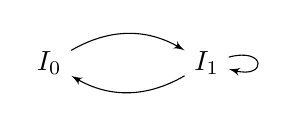
\begin{tikzpicture}
\tikzset{edge/.style = {->,>=latex'}}
\node (a) at (0,0) {$I_{0}$};
\node (b) at (2,0) {$I_{1}$};

\draw[edge] (a)[bend left] to (b);
\draw[edge] (b)[bend left] to (a);
\draw[edge] (b)[loop right] to (b);
\end{tikzpicture}
\end{center}
On which the N-cycle follows the allowed closed path.
\begin{center}
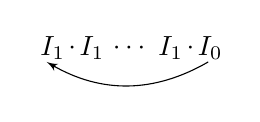
\begin{tikzpicture}
\tikzset{edge/.style = {->,>=latex'}}
\node (a) at (0,0) {$I_{1}$};
\node (b) at (0.5,0) {$I_{1}$};
\node (c) at (1.5,0) {$I_{1}$};
\node (d) at (2,0) {$I_{0}$};

\node (a1) at (-0.2,-0.1) {};
\node (d1) at (2.1,-0.1) {};

\draw[edge] (d1)[bend left] to (a1);
\path (a) to node {$\cdot$} (b);
\path (b) to node {$\cdots$} (c);
\path (c) to node {$\cdot$} (d);

\end{tikzpicture}
\end{center}
\example\ If there is a 4-cycle with
\[ x_1 = F(x_4)\,<\,x_3 = F(x_2) \,<\, x_2 = F(x_1) \,<\, x_4 = F(x_3) \]
Let $I_{\alpha} = [x_1,x_3]$, $I_{\beta} = [x_3,x_2]$, 
$I_{\gamma} = [x_2, x_4]$. Then
\[ F(I_{\alpha}) \supseteq I_{\gamma} \qquad 
F(I_{\beta}) \supseteq I_{\beta} \cup I_{\gamma} \qquad 
F(I_{\gamma}) \supseteq I_{\alpha} \]
\begin{center}
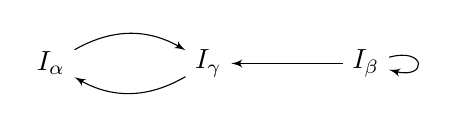
\begin{tikzpicture}
\tikzset{edge/.style = {->,>=latex'}}
\node (a) at (0,0) {$I_{\alpha}$};
\node (c) at (2,0) {$I_{\gamma}$};
\node (b) at (4,0) {$I_{\beta}$};

\draw[edge] (a)[bend left] to (c);
\draw[edge] (c)[bend left] to (a);
\draw[edge] (b) to (c);
\draw[edge] (b)[loop right] to (b);
\end{tikzpicture}
\end{center}
There is a fixed point in $I_{\beta}$, a 2-cycle oscillating between 
$I_{\alpha}$ and $I_{\gamma}$, but no obvious way to find a 3-cycle or 5-cycle
etc.
These sorts of arguments can be used to prove the remarkable result.
\\
\\
\theorem\ Sharkovsky \\
If $F$ is a continous map $\mathbb{R} \to \mathbb{R}$, $F$ has an N-cycle
and $N \rhd n$ with respect to the following ordering, then $F$ has an n-cycle.
\begin{equation*}
\begin{array}{c}
3 \rhd 5 \rhd 7 \rhd 9 \rhd \cdots \\
\rhd 2\cdot3 \rhd 2\cdot5 \rhd 2\cdot7 \rhd 2\cdot9 \rhd \cdots \\
\rhd 2^2\cdot3 \rhd 2^2\cdot5 \rhd 2^2\cdot7 \rhd 2^2\cdot9 \rhd \cdots \\
\vdots \\
\rhd 2^i\cdot3 \rhd 2^i\cdot5 \rhd 2^i\cdot7 \rhd \cdots \\
\vdots \\
\rhd 2^i \rhd 2^{i-1} \rhd \cdots \rhd 4 \rhd 2 \rhd 1 \\
\end{array}
\end{equation*}
Proof: Not in course.
\\
\\
E.g. 
\begin{itemize}
\item 3-cycles $\implies$ cycles of all order (already proved)
\item 4-cycles $\implies$ 2 cycles \& fixed point regardless of order 
      $x_1,\dots ,x_4$
\end{itemize}
\subsection{The Tent Map}
\[ x_{n+1} = \left\{ \begin{array}{ccc} 
\mu x_n & \mbox{for} & 0 \leq x_n \leq \frac{1}{2} \\
\mu (1-x_n) & \mbox{for} & \frac{1}{2} \leq x_n \leq 1
\end{array} \right. \]
This only maps $[0,1]$ into itself if $0 \leq \mu \leq 2$. There is always a
fixed point at $x=0$, which is stable for $\mu < 1$ (dull) and unstable
for $\mu >1$.
\\
\\
For $1 < \mu \leq 2$ there is another fixed point where 
$\displaystyle x_0 - \mu(1-x_0) \implies x_0 = \frac{\mu}{1+\mu} > \frac{1}{2}$
which is always unstable (because $F'(x_0)=-\mu < -1$).
\\
\\
The interesting range is $1<\mu\leq 2$ for which neither fixed points is an
attractor, and the orbits are bounded. We will show that $F$ is chaotic 
throughout this range.
\\
\\
We proceed to establish a horseshoe for $\mu>1$ in several steps:
\begin{enumerate}[1.]
\item Every orbit (apart from $x=0$) eventually enters and remains in the 
      interval \[A = [F^2(1/2),F(1/2)] = [\mu(1-\mu/2),\mu/2]\]
      \begin{proof} % The proof is a picture!
      Note: since $x_0$ is unstable, orbits can only reach the neighbourhood 
      of $x_0 = \frac{\mu}{1+\mu}$ if its preimage $x_{-1} = \frac{1}{1+\mu}
      \in A \implies \frac{1}{1+\mu} > \mu(1-\frac{\mu}{2}) \implies \mu^2 >2 $
      \end{proof}
\item Consider
      \[\arraycolsep=1.1pt\def\arraystretch{1.2} F^2(x)= \left\{ \begin{array}{lcrcl}
      \mu^2 x         &~\quad& 0        &\leq x \leq& 1/2\mu \\
      \mu(1-\mu x)    &~\quad& 1/2\mu   &\leq x \leq& 1/2 \\
      \mu(1-\mu(1-x)) &~\quad& 1/2      &\leq x \leq& 1-1/2\mu \\
      \mu^2(1-x)      &~\quad& 1-1/2\mu &\leq x \leq& 1 
      \end{array} \right. \]
      with $F(1/2\mu) = F(1-1/2\mu) = 1/2$. \\
      Let $x_{-2}$ be the preimage of $x_{-1}$ in $x>1/2$. $F^2(x_{-2})=F(x_{-1})
      = x_0$. Therefore 
     \[\mu(1-x_{-2}) = \frac{1}{\mu+1} \implies x_{-2} = 1 - 
     \frac{1}{\mu(1+\mu)} \]
\item Change of coordinates (renormalisation). $F^2$ acts on the intervals 
      $J_L = [x_{-1},x_0]$ and $J_R = [x_0, x_{-2}]$ like a tent map with
      parameter $\mu^2$. There are two cases:
      \begin{itemize}
      \item $\mu^2 \geq 2$.
            \[ F^2(1/2) = \mu(1-\frac{\mu}{2}) < x_{-1}=\frac{1}{1+\mu}\]
            \[ F(1/2) = \frac{\mu}{2} > x_{-2}=1-\frac{1}{\mu(1+\mu)}\]
            $F^2$ has horseshoes on both $J_L$ and $J_R$. $F$ is chaotic and
            the chaotic attractor is the whole of $A = [F^2(1/2),F(1/2)]$.
      \item $\mu^2 <2$ \\
            $F^2$ maps both of $J_L$ and $J_R$ into themselves, and there are
            attracting subintervals
            \[ A_L = [F^2(1/2), F^4(1/2)] \subset J_L\]
            \[ A_R = [F^3(1/2), F(1/2)] \subset J_R\]
            with $F(A_R)=A_L$, $F(A_L) \subseteq A_R$, $x_0 \not \in A_L \cup A_R$
      \end{itemize}
\item \theorem\ \\
      If $\displaystyle 2^{\frac{1}{2^{n+1}}} \leq \mu < 2^{\frac{1}{2^n}}$ then
      $F^{2^{n+1}}$ has a horseshoe, $F$ is chaotic and the chaotic attractor
      consists of $2^n$ intervals, which are permuted by $F$.
      \begin{proof} Apply arguments 1-3 inductively \end{proof}
\end{enumerate}
\subsection{The Logistic Map}
\[ x_{n+1} = \mu x_n ( 1- x_n) \]
Find numerically that there exists a period doubling cascade in 
$3<\mu<\mu_{\infty} =3.5700\cdots$ with $\mu_{\infty}-\mu_k \sim A \delta^{-k}$
as $k \to \infty$ with $\delta = 4.6692016\cdots$ There is chaos for 
$\mu_{\infty} < \mu \leq 4$. In this range there are ``windows'' of stable
N-cycles e.g. P3 in $1+\sqrt{8}=3.8284<\mu < 3.8415$
\\
\\
There exists period-doubling cascades of the N-cycles, e.g. P3$\to$P6$\to$P12 
etc. accumalating at $\mu_{\infty}^{(3)} = 3.8396$ with 
$\mu_{\infty}^{(3)}-\mu_k \sim B \delta^{-k}$ and the same $\delta$.
In fact, get the same $\delta$ for all maps with a quadratic maximum. Why?
\\
(Note: ``P3 $\implies$ Chaos'' so the chaotic sets are still there just not 
attracting.)
\end{document}
